\part{Holeyman}

\section{Equilibre limite d'un massif de sol}

    \subsection{Equilibre neutre des massifs horizontaux}

    Soit un ouvrage de soutènement quelconque : 
        \begin{multicols}{2}
            \begin{figure}[h!]
            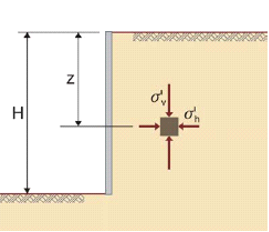
\includegraphics[scale=1]{Holeyman/images/H1.PNG}
            \caption{Contrainte sur une facette quelconque}
            \end{figure}
            \vfill\null\columnbreak
            \begin{figure}[h!]
            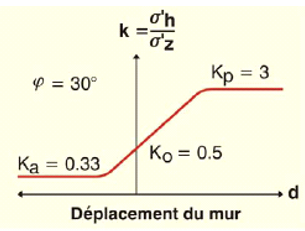
\includegraphics[scale=1]{Holeyman/images/H2.PNG}
            \caption{coefficient de pression des terres}
            \end{figure}
        \end{multicols}
    
    On détermine sa contrainte verticale s'exerçant sur une facette horizontale à une profondeur z :
    \medskip
    \begin{center}
    $\sigma_v = \gamma z$
    \end{center}
    On ne peut cependant pas déterminer la contrainte horizontal $\sigma_h$. On va devoir avoir recours au coefficient $K$, qui exprime le rapport entre la contrainte horizontale et la contrainte verticale. Autrement appelé le coefficient de pression des terres. Ce coefficient dépend de l'état du massif.
    
    \begin{itemize}
        \item L'état d'équilibre est neutre, si la paroi ne fait pas sentir sa présence.
        \item L'état est passif si la paroi compresse le massif sol. Après un certain déplacement, le sol atteint la butée ($K_p =$ coefficient de butée).
        \item L'état est actif si la paroi est déplacée par la détente du sol. Le sol est alors dit en poussée ($K_a =$ coefficient de poussée).
    \end{itemize}
    
    \medskip
    \underline{Observations} 
    
    \begin{itemize}
        \item Le déplacement de la paroi amenant le sol en butée est nettement plus important que celui nécessaire pour atteindre la poussée.
        \item Une fois l'état de poussée ou de butée atteint, le coefficient $K$ reste constant, la contrainte horizontale ne varie donc plus.
        \item Un sol en poussée à une contrainte horizontale plus faible qu'à l'état neutre, $K_a < K_0 < K_p$.
    \end{itemize}
        
    On peut à présent calculer la contrainte horizontale si on a à notre disposition la valeur de $K_0$. Pour se faire il existe trois méthodes :
    
    \subsubsection{Hypothèse de comportement élastique}
    
        Dans cette première approche, on considère le sol comme un matériau élastique isotrope caractérisé par son module de Young et son coefficient de Poisson. 
        Nous somme en présence d'un sol élastique, pour exprimer la condition "oedométrique", il faut utiliser la loi de Hooke à trois dimensions :
        
        \begin{center}
            \begin{tabular}{cc}
                $\epsilon_x = \frac{1}{E}[\sigma_x - \nu (\sigma_y + \sigma_z)] = 0$ \: \: &
                $\epsilon_y = \frac{1}{E}[\sigma_y - \nu (\sigma_x + \sigma_z)] = 0$
            \end{tabular}
        \end{center}
        
        Le massif est semi-infini horizontal, on a donc bien une déformation nulle horizontalement. Les contraintes selon X et selon Y sont donc égale. En résolvant ce système, on obtient que :
        
        \begin{center}
            $\sigma'_h = \frac{\nu}{1-\nu} \sigma'_v$
        \end{center}
        
        On observe: $K_0 = \frac{\nu}{1-\nu}$ (élastique) 
        
        On cherche ensuite à évaluer \textbf{le module oedométrique $E_0$}. Il s'agit du rapport entre la contrainte et la déformation verticale. On refait donc appel à la loi de Hooke à trois dimensions et on y introduit la contrainte verticale grâce à son rapport trouvé précédemment avec les contraintes horizontales. On obtient ainsi :
        
        \begin{center}
            $E_0 = \frac{(1-\nu)E}{(1-2\nu)(1+\nu)} = \frac{1}{m_v}$
        \end{center}
        
        Le module oedométrique peut être vu comme l'expression de la raideur verticale d'un matériau confiné latéralement. 
        
        Supposons à présent que nous avons une contraintes sphérique et donc semblable dans toutes les directions, les déformations engendrées seront donc les mêmes dans toutes les directions également. On définira ainsi le \textbf{module de compressibilité} (volumique) :
        
        \medskip
        \begin{center}
        \begin{tabular}{c|c}
            $B = \frac{P}{\epsilon-v} = \frac{E}{3(1-2\nu)}$  &  p: contrainte sphérique  \\
                          &  $\epsilon_v$: somme des déplacements en X,Y et Z 
        \end{tabular}
        \end{center}
        
        
    \subsubsection{Approche expérimentale}
    
        Il faut dériver tout sol normalement consolidé (expérimentalement). On obtient une expression de $K_0$ en fonction de l'angle de frottement interne $\phi$. Egalement appelé formule de Jacky.
        
        \begin{center}
            $K_0 (NC) \approx 1 - \sin \phi$
        \end{center}
        
    \subsubsection{Encadrement entre limites}
    
        Les deux méthodes précédentes permettent de dégager certaines tendances. D'une part la théorie élastique encadre ces valeurs dans l'intervalle [0 ; 1] et la donne en fonction d'un unique paramètre, le coefficient de Poisson. D'autre part l'approche expérimentale nous donne le coefficient de pression par rapport à l'angle de frottement interne de rupture du sol. On obtient donc des observations comprises dans l'intervalle [0.25 ; 1]. Ce qui correspond en pratique à des angles variant de $45°$ à $0°$. 
        
        Cette dernière méthode consiste à définir deux états limites et considérer que l'état du sol actuel est compris dedans. Ces deux états limites sont :
        
        \begin{itemize}
            \item La mise en rupture du sol lorsque $K$ décroit depuis $K_0$ (plastification par étalement horizontal du sol)
            \item La mise en rupture du sol lorsque $K$ croit depuis $K_0$ (plastification vertical par empilement)
        \end{itemize}
        
        Dans le point suivant nous verrons les différentes techniques pour calculer ces deux limites.
        
    \subsection{Limites inférieure et supérieure pour un massif horizontal}
    
        \begin{itemize}
            \item \textbf{A l'état neutre:} le sol est en équilibre, il n'y dès lors pas de rupture possible. Le cercle n'est donc pas tangent aux droites intrinsèques.
            \item \textbf{A l'état actif (en poussée):} la contrainte verticale reste inchangée (car même quantité de sol) mais la contrainte horizontale diminue. Si la diminution est trop importante, il y a rupture.
            \item \textbf{A l'état passif (en butée):} la contrainte verticale reste toujours constante mais la contrainte horizontale augmente. Cette fois, une trop grande augmentation entraîne la rupture.
        \end{itemize}
        
        \begin{multicols}{2}
            \begin{figure}[h!]
            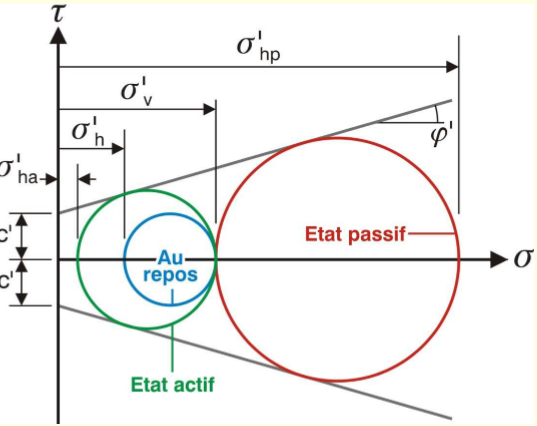
\includegraphics[scale=0.5]{Holeyman/images/H3.PNG}
            \caption{Evolution de l'équilibre}
            \end{figure}
            \vfill\null\columnbreak
            \begin{figure}[h!]
            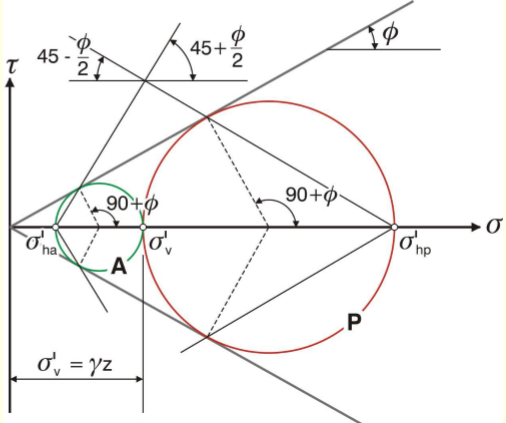
\includegraphics[scale=0.5]{Holeyman/images/H4.PNG}
            \caption{Equilibres limites}
            \end{figure}
        \end{multicols}
        
        \subsubsection{Etats limites pour un sol pulvérulent ($C' = 0$)}
            En étudiant la géométrie du cercle, on trouve : $\sigma_1 (1 -\sin \phi) = \sigma_3 (1 + \sin \phi)$. 
            La suite de la réflexion diffère selon que l'on cherche l'expression de $K_a$ ou de $K_p$ :
            
            \begin{center}
            \begin{tabular}{c | c}
                \textbf{Butée :} & \textbf{Poussée :} \\
                    On recherche la contrainte maximum & On recherche la contrainte minimu \\
                     et donc on s'intéresse à $\sigma_1$  & 
                     et donc on s'intéresse à $\sigma_3$ \\
                    $\sigma_1 = \sigma'_h$ & $\sigma_3 = \sigma'_h$ \\
                    $\sigma_3 = \sigma'_v$ & $\sigma_1 = \sigma'_v$ 
            \end{tabular}
            \end{center}
            
            Grâce à la trigonométrie, nous savons que :
            
            \begin{center}
            \begin{tabular}{c|c}
                $\tan(\frac{\pi}{4}+\frac{\phi}{2}) = \sqrt{\frac{1+\sin \phi}{1-\sin \phi}}$ \: \:&
                $\tan(\frac{\pi}{4}-\frac{\phi}{2}) = \sqrt{\frac{1-\sin \phi}{1+\sin \phi}}$ \\
            \end{tabular}
            \end{center}
            
            On obtient un rapport entre $\sigma'_h$ et $\sigma'_v$, et donc $K_p$ et $K_a$ :
            
            \begin{center}
            \begin{tabular}{c|c}
                $K_p = \frac{\sigma'_{h,max}}{\sigma'_v} = \tan^2(\frac{\pi}{4}+\frac{\phi}{2})$ \: \:&
                $K_a = \frac{\sigma'_{h,min}}{\sigma'_v} = \tan^2(\frac{\pi}{4}-\frac{\phi}{2})$ 
            \end{tabular}
            \end{center}
            
        \subsubsection{Calcul de $\sigma'_{h(min)}$ (poussée) selon Rankine ($C > 0$)}
        
            Cette méthode fait pour hypothèse que le massif situé au dessus de la surface de glissement est à l'équilibre. Nous somme donc dans le cas ci-dessous : 
            
            \begin{figure}[h!]
            \center
            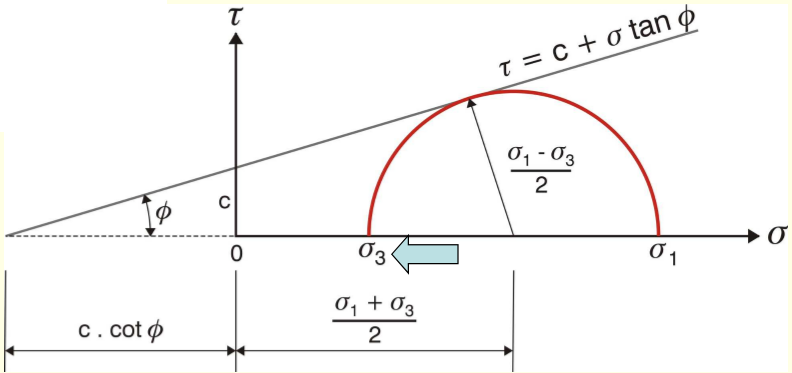
\includegraphics[scale=0.7]{Holeyman/images/H5.PNG}
            \end{figure}
            
            Comme précédemment, on exprime $\sigma_1$ et $\sigma_3$ par rapport à l'angle $\phi$ (par une étude trigonométrique du triangle ADC) et on le simplifie de la même manière que précédemment. Seul le cas minimum nous intéresse donc on considère :
            
            \begin{center}
            \begin{tabular}{cc}
                $\sigma_3 = \sigma'_{h(min)}$ \: \:&
                $\sigma_1 = \sigma'_v$ 
            \end{tabular}
            \end{center}
            
            En se basant sur la valeur de $K_a$ obtenue précédemment (en sol pulvérulent) on obtient :
            
            \begin{center}
                $\sigma'_{h,min} = \sigma'_v K_a - 2 c \sqrt{K_a}$
            \end{center}
        
        \subsubsection{Calcul de $\sigma'_{h(max)}$ (butée) selon Rankine ($C > 0$)}
        
            Même shéma que précédemment et même résolution trigonométrique, mais cette fois on s'intéresse au cas maximum donc : 
            
            \begin{center}
            \begin{tabular}{cc}
                $\sigma_1 = \sigma'_{h(max)}$ \: \:&
                $\sigma_3 = \sigma'_v$ 
            \end{tabular}
            \end{center}
            
            En se basant sur la valeur de $K_p$ obtenue précédemment (en sol pulvérulent) on obtient :
            
            \begin{center}
                $\sigma'_{h,max} = \sigma'_v K_p + 2 c \sqrt{K_p}$
            \end{center}
            
        \subsubsection{Observations}
        
            \begin{itemize}
                \item $K_0$ est généralement inférieur à 1 et proche de $K_a$
                \item Pour des angles de frottement moyens ($\phi = 30°$) $K_p \approx 10 K_a$
                \item Lorsque l'angle de frottement et la cohésion sont nuls, on retrouve une condition hydrostatique: $K_0 = K_a = K_p = 1$
                \item $K$ ne s'applique qu'aux contraintes effectives (on ne considère pas la contrainte interstitielle). La contrainte latérale totale s'obtient donc par la formule: $\sigma_h = \sigma'_h + u$
            \end{itemize}
            
    \subsection{Massif à l'état Neutre}
            
        \begin{figure}[h!]
            On considère ici un massif sol sec semi-infini et limité par un plan incliné de pente $i$.
            \center
            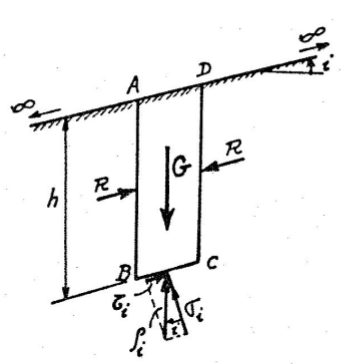
\includegraphics[scale=1]{Holeyman/images/H6.PNG}
            \caption{Elément de volume d'un talus infini}
        \end{figure}
            
        \begin{itemize}
            \item toute facette verticale d'un massif semi-infini est indifferenciable d'une autre
            \item Par symétrie les forces $R$ s'équilibre puisque le talus est de longueur infinie
        \end{itemize} 
        
        Si le talus est en équilibre, il peut arriver à la limite de deux façons différentes, soit en exerçant sur le massif une détente uniforme, soit une compression uniforme. 
        
        Nous allons analyser ces cas limites avec et sans cohésion. Soit dans le cas pulvérulent ($C = 0$) et dans le cas cohérent ($C \ne 0$).
        
        \begin{center}
               \textit{"Pour les deux points suivant, il est préférable de bien comprendre les cercles de Mohr"}
        \end{center}
        
        \subsubsection{Cas pulvérulent}
        
            On suppose que l'on connaît les contraintes s'exerçant sur une facette parallèle à la pente du talus $S = (\sigma_1, \tau_1)$ 
            
            On sait donc que le pôle se trouve sur la droite de la pente $i$ passant par $S$. Cela nous laisse encore une infinité de cercle possible. Il faut poser une condition complémentaire. 
            
            \underline{Si $i = \phi'$:} 
            Dans ce cas particulier nous avons : 
            
            \begin{center}
            \begin{tabular}{cc}
                $p = p'$ \: \: & $K_0 = K_a = K_p = K_1$ 
            \end{tabular}
            \end{center}
            
            Comme $i=\phi'$, le point $S$ se trouve forcément sur une des droite de Coulomb, on ne peut donc plus que tracer un seul cercle passant par $S$ et tangent aux deux droites de Coulomb (On considère le talus à la limite de son équilibre).

            \begin{figure}[h!]
            \center
            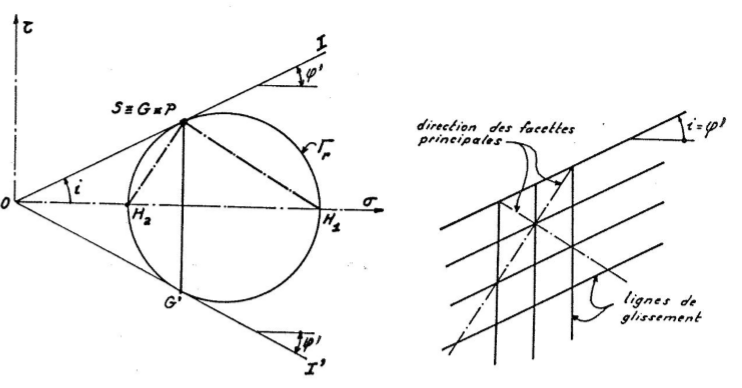
\includegraphics[scale=0.7]{Holeyman/images/H7.PNG}
            \caption{Cercle de Mohr à l’état pulvérulent avec $i=\phi'$ }
            \end{figure}
            
            On connaît les point $H_1$ et $H_2$ soit les croisements entre le cercle et l'axe des contraintes normales. On connaît ainsi nos contraintes principales majeure et mineure. 
            
            On obtient la direction des facettes principales par parallélisme avec $PH_1$ et $PH_2$ (toujours perpendiculaire entre elles). On obtient pour finir les lignes de glissement par parallélisme avec $OP$ et $PG'$. 
            
            \underline{Si $i < \phi'$:} 
            
            Le point S se trouve à l'intérieur de l'angle formé par les droites de Coulomb. On peut dessiner une infinité de cercle de Mohr compris dans les limitations des droites de Coulomb. Il y a une infinité d'état d'équilibre possible.
            Ces états d'équilibres peuvent être rompus soit par compression du sol uniforme soit par détente uniforme. Pour chacun des cercles on peut trouver des états de contraintes correspondant à ces deux cas limites ($\Gamma_c$ et $\Gamma_d$). 
            
                \begin{figure}[h!]
                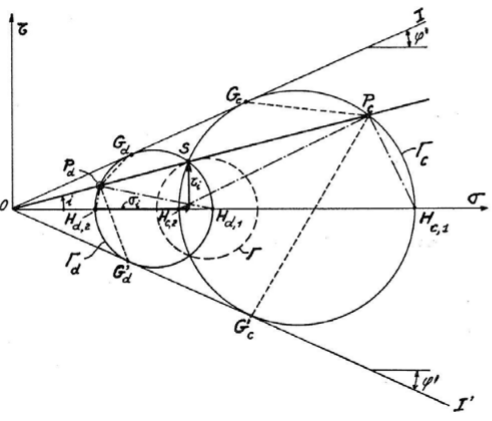
\includegraphics[scale=0.6]{Holeyman/images/H8.PNG}
                \caption{Cercles de Mohr à l’état pulvérulent avec $i < \phi’$ }
                \end{figure}
                
                \begin{figure}[h!]
                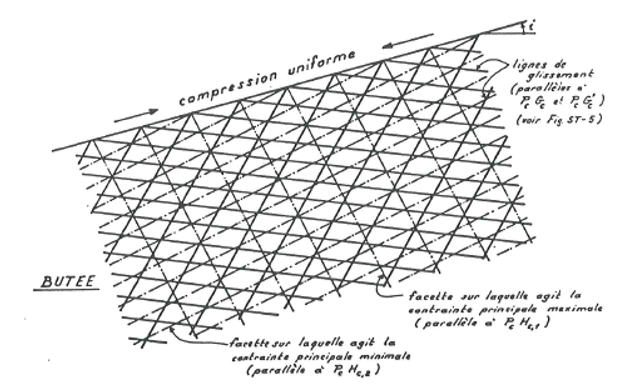
\includegraphics[scale=0.6]{Holeyman/images/H9.PNG}
                \caption{Réseau de lignes de glissement et directions des facettes principales}
                \end{figure}
            
            On trace ensuite les lignes parallèles pour trouver les lignes de glissements et la direction des facettes principales.
            
            \underline{Si $i > \phi'$:} 
            
            Equilibre impossible du talus.
            
        \subsubsection{Cas cohérent}
        
            Désormais, les droites intrinsèques (ou droites de Coulomb) ne passe plus par l'origine du diagramme. 
            
            \underline{Si $i \le \phi'$:} 
            
            Comme précédemment, on peut tracer une infinité de cercles. De plus, ici les droites OS, OI et OI' ne sont plus concourantes. Les directions des facettes ne sont donc plus indépendante de la profondeur. Les lignes de glissement et mes directions des facettes principales seront donc curvilignes. 
        
            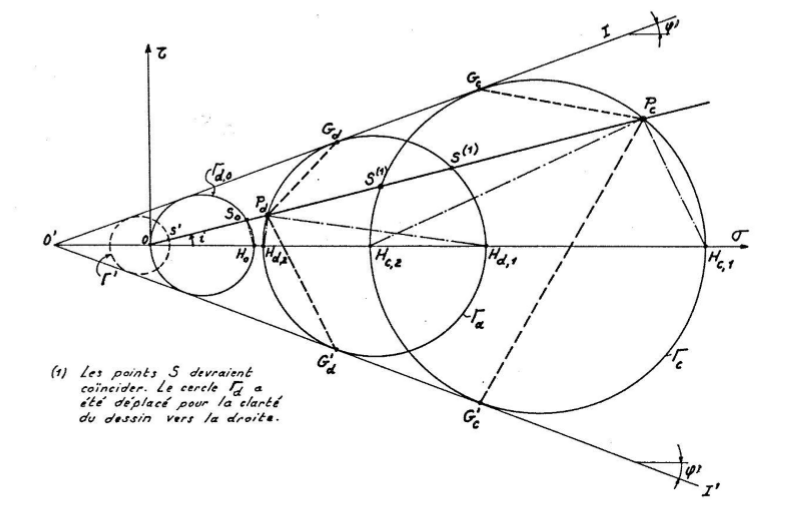
\includegraphics[scale=0.8]{Holeyman/images/H10.PNG}
            
            \begin{multicols}{2}
                Dans un cas de Compression :
                \begin{figure}[h!]
                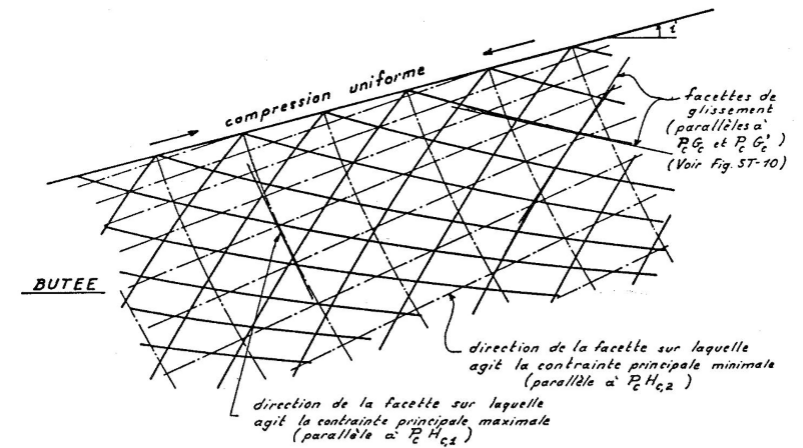
\includegraphics[scale=0.6]{Holeyman/images/H11.PNG}
                \caption{ Réseau de lignes de glissement et directions des facettes principales en butée }
                \end{figure}
            \vfill\null\columnbreak
                Dans un cas de Détente :
                \begin{figure}[h!]
                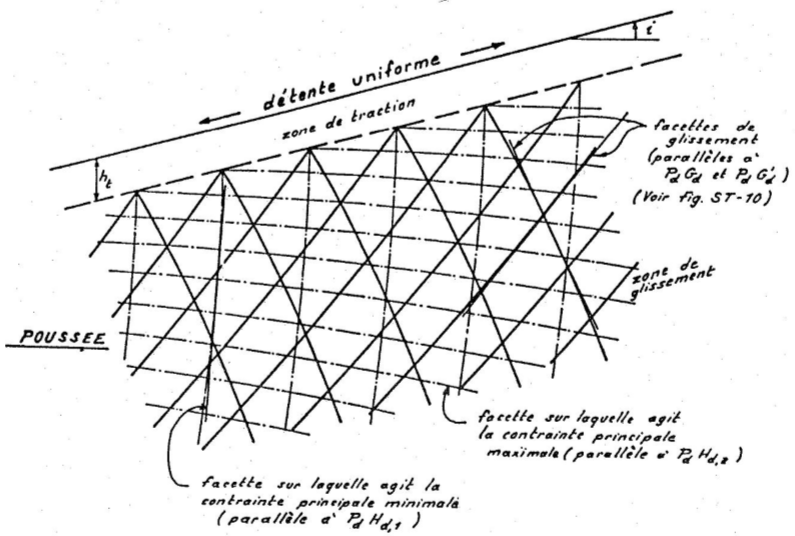
\includegraphics[scale=0.5]{Holeyman/images/H12.PNG}
                \caption{Réseau de lignes de glissement et directions des facettes principales en poussée}
                \end{figure}
            \end{multicols}
            
            Pour représenter le cas en détente, on peut dessiner les lignes de glissement qu'en dessous d'une certaine profondeur $h_t$. En effet, le point $S_0$ correspond à une profondeur telle que le cercle $R_{d,0}$ est tangent à l'axe des contraintes tangentielles $\tau$. Certaines facettes sont donc soumises à la traction. Or le mode de rupture par traction est différent de celui de compression. 
            
             \underline{Si $i > \phi'$:} 
            
            Situation impossible à réaliser, le talus n'est pas en équilibre.
            
\section{Reconnaissance géotechnique et Essais in situ}
    
    La reconnaissance géotechnique est essentielle dans le processus de conception géotechnique. Elle permet la caractérisation d'un site (info qualitative : type de sol, profondeur des nappes, ... et info quantitatives : angle de frottement, constante de compressibilité, ...). Pour avoir de bonnes informations, elles sont généralement traitées sur le terrain et en labo (in situ).
        
    \subsection{Forages}
        
        Cela permet d'étudier la nature d'un sol, définir sa stratigraphie (épaisseur des différentes couches) et permet de ramener des échantillons remaniés ou non. Si l'échantillon est remanié on peut en tirer des caractéristiques physiques (granulométrie, nature du sol, ...). Si il ne l'est pas, des caractéristique mécaniques (compressibilité, degré de pré-consolidation,...). 
            
        Il existe deux types de forage : par injection d'eau ou à sec. Le premier permet de creuser un trou et de remonter des boues (mélange de différentes couches) il convient généralement pour le placement de tube piézométrique. Le deuxième permet de ramener des échantillons sans mélanger le sol. 
            
        Dans le cas d'extraction d'échantillons remaniés (non représentatif structurelement et mécaniquement), on utilise une tarière (à vrille ou à cuillère pour sol cohérent, à clapet ou à boulet). Si le sol n'est pas cohérent, il aura tendance à se refermer, il faut donc soutenir les parois.
            
        Durant un forage, un chef foreur établi un "état d'ouvrage" qui reprend en tableau toutes les infos spécifiques utiles (date et heure du prélèvement, diamètre de forage, utilisation ou non de fourreaux, nature, consistance, ...). 
            
        Pour obtenir des infos précises sur la nature du sol, le forage est interrompu pour prélever des échantillons (On réalise donc un examen en temps réel des couches rencontrées). 
            
        Il est possible de prendre des échantillons très peu remanié. Deux techniques sont utilisées. L'utilisation d'un anneau volumétrique ou par découpage in situ (dans le cas d'un matériaux très cohérent) Le principe est le même dans les deux cas, "isoler" une partie du sol et retirer ce qu'il y a autour pour garder un échantillon final intouché. Dans le cas de prélèvement en profondeur, on utilisera un carottier qu'on placera dans un trou de forage. On peut exprimer le degré géométrique de remaniement d'un carottier par la formule suivante (qui dépend des diamètres) : 
            
        \begin{center}
                $C_a = 100 \frac{d^2_e - d^2_i}{d^2_i}$
        \end{center} 
            
        \subsubsection{Présence d'une nappe phréatique}
            
            La présence d'une nappe phréatique lors d'un forage peut avoir différentes conséquences. Lorsque la pression d'eau dans le tubage est inférieur à la pression interstitielle, le gradient hydraulique à l'intérieur est ascendant, l'eau a tendance à s'introduire dans le tube. A l'inverse, si la pression dans le tube est supérieur à la pression interstitielle, il y a un écoulement vers le bas. On peut donc contrecarrer la remontée de sol en augmentant la pression.
            
            Supposons que l'on égalise la pression dans le tube à la pression interstitielle. Lorsque le forage traverse la couche imperméable, la couche de sable sous-jacente si elle n'est pas saturé, absorbe une partie de l'eau du tubage. On observe une brusque diminution du niveau d'eau dans le trou de forage. Ce qui  indique la présence d'une nappe perchée. 
            
            Supposons maintenant que cette nappe piégée sous la couche imperméable soit une nappe captive, lorsque le forage traverse la couche imperméable, on observe une brusque remontée d'eau.
            
        \subsubsection{Plan d'un piézomètre}
            
                \begin{figure}[h!]
                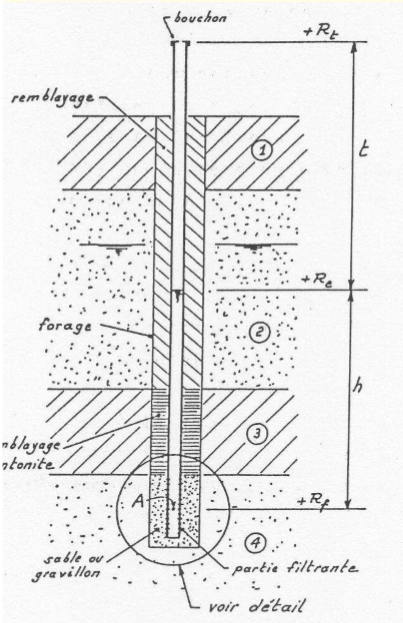
\includegraphics[scale=0.8]{Holeyman/images/H13.PNG}
                \end{figure}
        

                \begin{figure}[h!]
                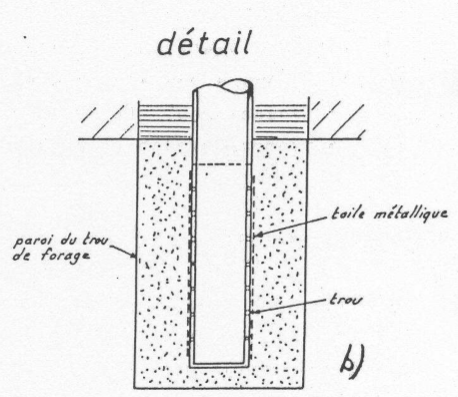
\includegraphics[scale=1]{Holeyman/images/H14.PNG}
                \end{figure}
            
        \subsection{Sondage et diagraphie}
            
            Les forages sont lent et coûteux, pas toujours évident à mettre en oeuvre et peu précis si pas assez nombreux (petit échantillon pour une grande zone). De plus on s'intéresse à des informations concernant les caractéristiques mécaniques du sol plutôt que physique (échantillons non remaniés). Il peut donc s'avérer plus intéressant de réaliser des sondages (Processus par lequel un instrument, appelé 
            sonde est introduit dans un milieu pour en rapatrier les propriétés). 
            
            Une diagraphie est un diagramme représentant, de façon quasi continue, une ou plusieurs caractéristiques du sol en fonction d'une coordonnée, en l'occurrence la profondeur. 
            
            Un essai de pénétration permet de caractériser par une diagraphie la résistance mécanique du sol et idéalement d'inférer la nature du sol par corrélations.
            
            \begin{itemize}
                \item Sans forage :
                \begin{itemize}
                    \item pénétration statique au cône (CPT) : sols meubles
                    \item pénétration dynamique (DPB) : sols à forte résistance
                \end{itemize}
                
                \item Avec forage :
                \begin{itemize}
                    \item pénétration standard (SPT)
                    \item pénétration dynamique (DPA) : sols à forte résistance
                \end{itemize}
            \end{itemize}
            
        \subsubsection{Essais de pénétration statique au cône mécanique (CPT)}
            
            Méthode qui consiste à enfoncer une pointe dans le sol à vitesse quasi statique (2cm/sec) et ainsi mesurer l'effort d'enfoncement. 
            
            \begin{multicols}{3}
            
                \begin{figure}[h!]
                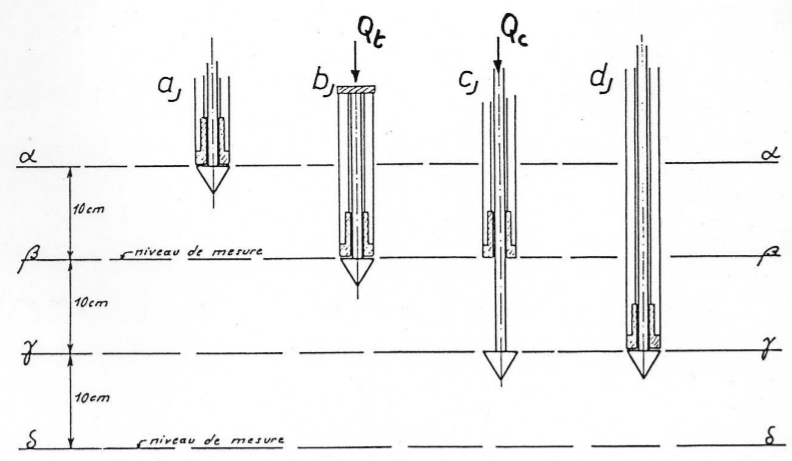
\includegraphics[scale=0.65]{Holeyman/images/H15.PNG}
                \end{figure}
            
            \vfill\null\columnbreak
            \vfill\null\columnbreak
            
                \begin{figure}[h!]
                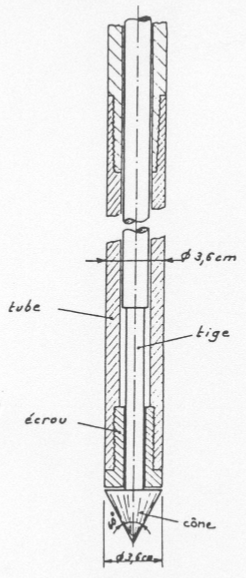
\includegraphics[scale=0.6]{Holeyman/images/H16.PNG}
                \end{figure}
                
            \end{multicols}
            
            Le procédé est simple, on enfonce la tige de 10 cm dans le sol, on mesure $Q_t$ ensuite on enfonce le cône seul de 10 cm, on mesure $Q_c$. On ramène ensuite le tube contre le cône et on répète les étapes précédentes.
            
            On obtient par différence le frottement latéral global du sol traversé agissant sur l'extérieur du train de tubes : 
            
            \begin{center}
                $Q_{st} = Q_t - Q_c$ 
            \end{center}
            
            On défini la résistance unitaire à la pointe: $q_c = \frac{Q_c}{A_c} [MPa]$
            
            Grâce à ces tests, on peut calculer le pouvoir portant et le tassement du sol, estimer la cohésion de l'angle de frottement mais aussi avoir une idée de la profondeur d'une nappe d'eau et finalement connaître la nature du sol. 
            
            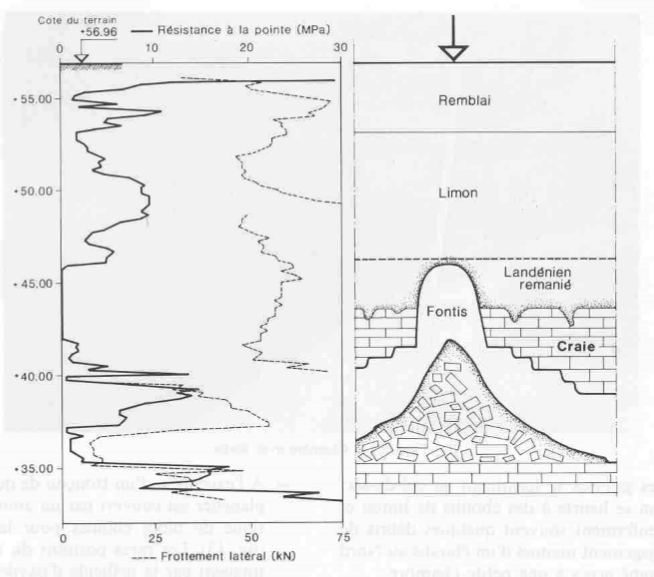
\includegraphics[scale=1]{Holeyman/images/H17.PNG}
            
            Ce même test peut être effectué de manière électrique, autrement appelé :
            
        \subsubsection{Essais de pénétration statique eléctrique (CPTE)}
        
            Le frottement unitaire $F_s$ est calculé le long du manchon ainsi que la résistance à la pointe $q_c$. Ces résultats sont calculés continuellement durant le test grâce au frottement unitaire on peut facilement déterminer l'indice de frottement $F_r$ du sol en présence et donc sa nature:
            
            \begin{center}
                \begin{tabular}{ccc}
                    $F_r = \frac{F_s}{q_c}100\%$ \: \: & Sable $\in [0; 2]\%$ \: \: & Argile $\in [3; 10]\%$
                \end{tabular}
            \end{center} 
            
            La différence avec le test précédent est qu'ici, la force est mesurée par des capteurs interne à la sonde et non présent dans le moteur faisant l'effort d'enfoncer le cône. Cela permet donc de prendre des mesures pendant l'enfoncement et non pas à intervalle régulier.
            
        \subsubsection{Essai de pénétration dynamique (DPT)}
        
            On a recours à ce genre d'essai dynamique lorsqu'un essai statique n'est pas possible (sol trop dur). Dans ce cas, au lieu d'enfoncer la sonde de façon quasi statique, on la fait pénétrer par battage, au moyen d'un mouton au poids déterminé que l'on laisse tomber d'une hauteur constante.
            
            Il en existe deux types : le A et le B. Le type A est effectué dans un forage, dès lors il ne subit pas de frottement entre le train de tige et le sol. Dans le type B, on prend un diamètre de pointe plus grand pour diminuer le frottement. On peut néanmoins l'estimer en évaluant la force nécessaire pour la mise en rotation du train de tiges.
            
            On établit alors un diagramme reprenant le nombre de coups en fonction de la profondeur (on va jusqu'à 20 mètres).
            
            On établit la résistance au cône dynamique sur base des considérations énergétiques :
    
            \medskip
            \begin{center}
            \begin{tabular}{c|c}
                $q_d = \frac{Mgh}{Ae}$ \: \:  &  e: pénétration moye,,e de la pointe par coup [cm]  \\
                          &  h: hauteur de la chute [m] 
            \end{tabular}
            \end{center} 
            
            Ex: DPB "lourd" utilise une masse de 63.5 Kg, une hauteur de chute de 75 cm et une pointe de 51mm de diamètre ($A_c = 20 cm^2$).
            
        \subsubsection{Essai de pénétration standart (SPT)}
        
            Cet essai est très similaire au précédent, à ceci près qu'il permet de prélever des échantillons du sol. Il consiste à enfoncer dynamiquement au fond d'un trou de forage un carottier aux dimensions normalisées. on regarde le nombre de coup nécessaire pour obtenir l'enfoncement voulu (généralement exprimé en pued). On peut ensuite étudier la carotte et ainsi avoir des renseignements physiques et mécaniques.
            
    \subsection{Essais in Situ}
        
        \subsubsection{Scissomètre}
        
            Il s'agit d'un dispositif cruciforme qui est enfoncé par pression statique dans le sol. On lui applique une rotation à vitesse angulaire constante. La rotation des ailettes crée un couple qui entraîne le cisaillement du sol. On mesure ensuite le couple $T$ nécessaire à cette rotation et on l'exprime en fonction de la géométrie du dispositif et de la cohésion non drainée du sol cohésif testé.
            
            \begin{center}
                $T=\frac{\pi d^3}{2} (\frac{h}{d}+\frac{1}{3})c_u$
            \end{center}
            
            On adapte la taille de l'ailette en fonction de la consistance de l'argile. Ce dispositif ne peut être utilisé que dans le cas de sols caractérisé par un seul paramètre de cisaillement, son usage est donc restreint aux sols cohésifs, faute de quoi l'estimation de $C_u$ serait grossièrement erronée.
            
        \subsubsection{Pressiomètre}
            
            On réalise un forage, y introduit un pressiomètre, le gonfle à pression définie et en mesure l'expansion. La sonde pressiométrique descend par palier en progression linéaire. A chaque palier de pression, on mesure le volume de la cellule en fonction du temps. On obtient ainsi une mesure de la pression $P_m$ lue au manomètre et une mesure du volume $V_m$ lue à l'indicateur de niveau. On porte enfin ces mesures sur un diagramme reprenant la pression appliquée dans la cellule $P_c$ en abscisses et l'accroissement de son volume $V_c$ en ordonnées.
            
            le graphe obtenu se divise en trois phases de déformation : %ajouter le graphe%
            \begin{itemize}
                \item phase 1: résorption du jeu entre forage et cellule jusqu'à mise en contact de la cellule avec la paroi du forage
                \item phase 2: déformation pseudo-élastique
                \item phase 3: plastification
            \end{itemize} 
            
            L'interprétation permet de déterminer le module de déformation ainsi qu'une pression limite avant rupture du sol (expansion de la cavité). 
            
            Un essai pressiométrique fait dans un sol trop peu cohérent est souvent accompagné d'un essai scissométrique au risque d'être imprécis.
            
    \subsection{Reconnaissance géophysique}
    
    Les méthodes de reconnaissance géophysique permettent de déterminer la nature et la profondeur des couches en se basant sur leur caractéristiques magnétiques, gravimétriques, sismiques ou électriques. 
        Patience, c'est pour le cours de l'année prochaine ça !
        
\section{Fondation superficielles (portance)}
    
    La capacité porta te d'une fondation résulte de la capacité du sol sous-jacet à supporter une charge sans subir de déformation excessives ni être mis en rupture par cisaillement. Une fondation superficielle ou "directe" est utilisée lorsque la base de l'ouvrage présente un pouvoir porta t insuffisant.
    
    Il existe différents types de fondation :
    \begin{itemize}
        \item Semelle isolée: Chaque colonne reporte la charge individuellement sur une semelle (forme carré, rectangulaire ou circulaire).
        \item Semelle filante: De forme rectangulaire, on l'utilise lorsque la charge à transmettre est répartie le long d'une ligne.
    \end{itemize}
    
    Lorsque la densité de colonnes et murs devient importante ou que le sol est médiocre, on utilise des fondations en grillage (croisement de semelle filante) ou en radier (mélange de semelle filante et isolée).
    
    Le dimensionnement de ces fondations est établi en fonction de la nature et des caractéristiques du sol rencontré ainsi que l'importance des charges à transmettre
    (Exemple de raisonnement P4 PDF fondations superficielles 2015).
    
    L'enfoncement $S$ d'une fondation accusant une charge $Q$ verticale croissante \textbf{si le sol est compacte} (dense ou raide) suivra trois phase :
    
    \begin{figure}[h!]
        \centering
        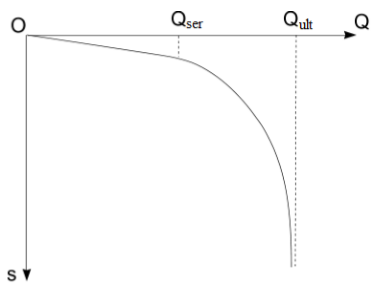
\includegraphics[scale=0.5]{Holeyman/images/H18.PNG}
    \end{figure}
    
    \begin{itemize}
        \item Courbe de mise en charge relativement linéaire. Principalement due à une compression du sol et une réduction du volume des vides.
        \item Les incrément de déformation augmente, il y a toujours une diminution des vides mais également des déplacements latéraux. On commence à atteindre localement la résistance au cisaillement.
        \item Une faible augmentation de charge entraine un enfoncement important, la rupture du sol par cisaillement se produit sous la charge ultime $Q_{ult}$.
    \end{itemize} 
    
    \textbf{Si le sol n'est pas assez compact}, on observe dès la première phase des déformations excessives par compression.
    
    La charge ultime n'est pas une constante pour un sol donné. Elle dépend des dimensions des fondations et des caractéristiques du sol intrinsèque, de l'inclinaison, des nappes phréatiques, ...
    
    Tout dimensionnement exige deux vérifications:
    \begin{itemize}
        \item Limites ultimes (ELU): Cette vérification concerne la rupture que l'on doit éviter (charge admissible suffisamment faible par rapport à la charge ultime).
        \item Limite de service (ELS): Cette vérification concerne les tassements (déformations inférieur à certaines limites imposées en fonction de l'ouvrage et du sol). Les fondations ne sont jamais chargées jusqu'à leur état ultime $Q_{ult}$, on se limite au pouvoir portant de service $Q_{serv}$ estimé avec un coefficient de sécurité approprié ($FS = 2$ ou $3$).
    \end{itemize}
    
    \begin{center}
        $FS = \frac{Q_{ult}}{Q_{serv}}$
    \end{center}
    
    On peut observer que le coefficient est très loin de ceux appliqué pour la stabilité des talus. Le choix du coefficient dépend du problème considéré, d'un arbitrage professionnel intégrant l'analyse à posteriori en cas de rupture ainsi qu'un rapport coût/sécurité.
    
    Il faudra encore vérifier si le tassement reste admissible sous la charge de service. Ce tassement est défini spécifiquement pour le projet. A l'équilibre limite de la déformation, la charge $Q_{lim}$ appliqué au sol provoque des déformations compatibles avec la stabilité. Certain cas iront jusqu'à même admettre l'endommagement partiel de l'ouvrage. Au final, la charge admissible sera calculée grâce à cette équation:
    
    \begin{center}
        $Q_{adm} \le min \{Q_{serv} = \frac{Q_{ult}}{F}; Q_{lim}\}$
    \end{center}
    
    \subsection{Mécanisme de rupture}
    
        Le phénomène de rupture du sol est généralement lié à une contrainte de cisaillement excessive. Il existe plusieurs théories et modèles pour évaluer la charge de rupture d'un massif de sol sous une fondation. On est cependant toujours amené à poser une certain nombre d'hypothèses. C'est pourquoi il est impératif, lors d'un calcul de fondation, d'exprimer très explicitement les hypothèses et les choix fait.
        
        Une hypothèse communément admise est celle d'un état plan de déformation. Cela permet de réduire le problème à deux dimensions, ce qui est pratique dans le cas d'un critère de rupture basé sur deux composantes (exemple: le critère de Mohr-Coulomb). Le problème se traite dans un plan sans oublier l'espèce physique, les unités ne change pas, même si elles dépendent d'éléments non représentés dans le plan. (Explication d'un problème type P8 PDF fondations superficielles 2015)
        
    \subsection{Coins de Rankine et forme canonique}
    
        En admettant une surface de rupture simpliste, on obtient une expression dimensionnellement correcte. L'équation en découlant sert de modèle à des formules plus précises développées par après.
        
        Soit le cas suivant (semelle filante et sol pulvérulent): $q_{ult} = \frac{Q_{ult}}{B}$ [KPa]
        
        \begin{figure}[h!]
            \center
            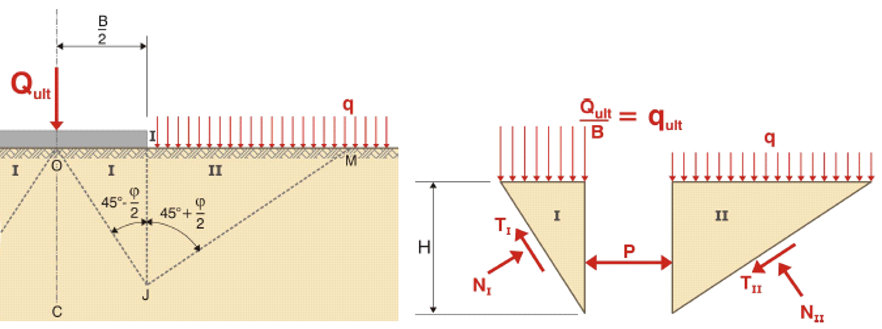
\includegraphics[scale=0.8]{Holeyman/images/H19.PNG}
            \caption{Mécanisme de rupture selon Rankine}
        \end{figure}
        
        La question qui se pose est de déterminer la contrainte uniforme verticale sur la fondation $q_{ult}$ menant à la rupture. Pour se faire, on suppose à la limite de rupture, le coin $I$ s'enfonce en poussant le coin $II$ vers l'extérieur. Ce mouvement est contrebuté par le coin $II$ qui devrait remonter latéralement et soulever la charge répartie $q$.
        
        On étudie la statique du problème: 
        \begin{center}
            \begin{tabular}{c|c}
                $ P_{I} = P_a = q_{ult}K_a H + \frac{\gamma}{2} H^2 K_a $ &  Force de poussée du coin $I$ \\
                $ P_{II} = P_q = qK_p H + \frac{\gamma}{2} H^2 K_p $ &  Force de butée du coin $II$ 
            \end{tabular}
        \end{center}
        
        L'équilibre de translation horizontal veut que $P_a = P_q$ et donc:
        \begin{center}
            $q_{ult} + \frac{1}{2} \gamma H = (q + \frac{1}{2} \gamma H) \frac{K_p}{K_a}$
        \end{center} 
        
        Avec un peu de trigonométrie on obtient:
        \begin{center}
            $H = \frac{1}{2} \tan(45° + \frac{1}{2} \phi) = \frac{1}{2} B \sqrt{K_p}$
        \end{center}
        
        On obtient finalement:
        \begin{center}
            $q_{ult} = q \frac{K_p}{K_a} + \frac{1}{2} \gamma (\frac{K_p}{K_a} - 1) \frac{B}{2} \sqrt{K_p}$
        \end{center}
        
        On doit maintenant tenir compte de la cohésion. Grâce au théorème des états correspondant de Caquot, en connaissant la solution pour un sol sans cohésion, on trouve la solution correspondante du sol avec cohésion en ajoutant la valeur "$c \cot \phi$" à chaque terme de contrainte normale:
        
        \begin{center}
            $F_c(\sigma, \tau, \phi, c) = F_p(\sigma*,\tau,\phi) = F_p(\sigma + c \cot \phi, \tau, \phi)$
        \end{center}
        
        \begin{figure}[h!]
            \center
            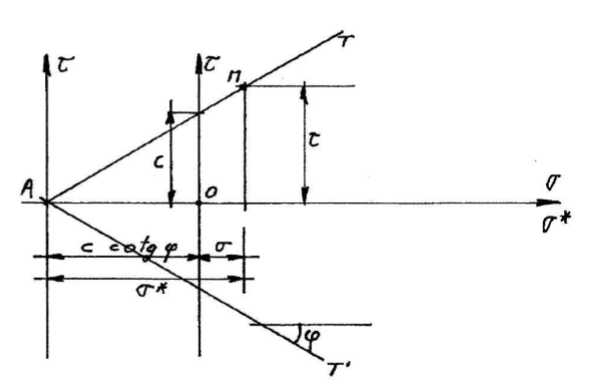
\includegraphics[scale=0.6]{Holeyman/images/H20.PNG}
            \caption{Etats correspondants de Caquot}
        \end{figure}
        
        Dans le cas d'un sol cohérent, l'équation devient donc:
        
        \begin{center}
            $q_{ult} + c \cot \phi = (q + c \cot \phi) \frac{K_p}{K_a} + \frac{1}{2}\gamma(\frac{K_p}{K_a} - 1) \frac{B}{2} \sqrt{K_p} \leftrightarrow q_{ult} = q \frac{K_p}{K_a} + c \cot \phi (\frac{K_p}{K_a} - 1) + \frac{1}{2} \gamma (\frac{K_p}{K_a}-1) \frac{B}{2} \sqrt{K_p}$
        \end{center} 
        
        On introduit ensuite les coefficients adimensionnels $N_q$, $N_c$ et $N_{\gamma}$ qui dépendent de l'angle de frottement interne $\phi$. On obtient alors la forme canonique de l'équation générale du pouvoir portant des fondations superficielles.
        
        \begin{center}
            \begin{tabular}{c|c}
                 $q_{ult} = qN_q + cN_c + \frac{1}{2} \gamma N_{\gamma}B$ 
                    &  $N_q$: terme de profondeur  \\
                    &  $N_c$: terme de cohésion  \\
                    &  $N_{\gamma}$: terme de surface 
            \end{tabular}
        \end{center} 
        
        Comme précisé précédemment, les développements ci-dessus sont basés sur des hypothèses trop simplistes qui négligent/violent certaines conditions:
        \begin{itemize}
            \item La surface de rupture observée en pratique n'est pas composée de deux segments de droites. le mécanisme de rupture décrit est non cinématiquement acceptable, le coin doit pénétrer dans le massif sous-jacent.
            \item Le cisaillement le long de l'interface entre les coins $I$ et $II$ n'est pas considéré. On ne prend en compte que l'équilibre horizontal au mépris de l'équilibre vertical de rotation.
        \end{itemize} 
        
        Ces critères font qu'on ne peut en pratique pas utiliser les coefficients de Rankine. Il nous suffira donc de garder la forme générale de la formule mais d'en changer les coefficients par d'autre valeurs obtenues avec des hypothèses plus réalistes.
        
    \subsection{Charge verticale centrée}
    
        Prandtl a établi une formule permettant de calculer le pouvoir portant limite d'une fondation de largeur B et de longueur infinie reposant sur un sol sans poids propre. Cette formule a été complétée par Buisman dans l'hypothèse d'un sol pesant.
        
        \subsubsection{Théorie de Prandtl - Buisman}
        
            \underline{Formule de Prandlt:} 
            
            Hypothèses : \begin{itemize}
                \item problème bidimensionnel
                \item sol est supposé sans poids propre
                \item sol incompressible (enfoncement uniquement dû au refoulement latéral par dépassement des contraintes de cisaillement)
                \item seules les déformations plastiques sont considéré (modifient pas la configuration géométrique car trop petites)
                \item $\tau_{max} = \sigma' \tan \phi$ (loi de Mohr-Coulomb)
                \item $\phi' = cst$ (néglige l'accroissement de la résistance)
                \item surface de contact entre la semelle et le sol est infiniment lisse ($\tau_{xz} = 0$)
                \item le sol situé au-dessus et à coté de la fondation ne possède pas de caractéristique de cisaillement (uniquement $q$ est pris en compte)
                \item on néglige la pression interstitielle ($u=0$)
                \item le mécanisme étudié est composé de deux triangles $I$ et $II$ es d'une spirale logarithmique $II$
            \end{itemize} 
            
            \begin{multicols}{2}
            
                \begin{figure}[h!]
                \center
                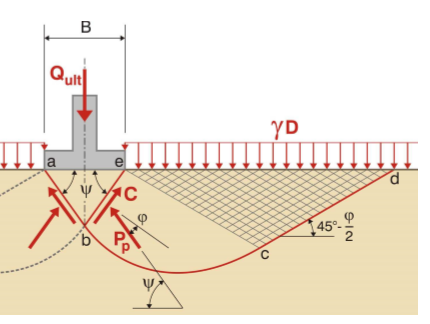
\includegraphics[scale=0.8]{Holeyman/images/H21.PNG}
                \caption{Mécanisme de rupture de Prandtl }
                \end{figure}
            
            \vfill\null\columnbreak
            
                \begin{figure}[h!]
                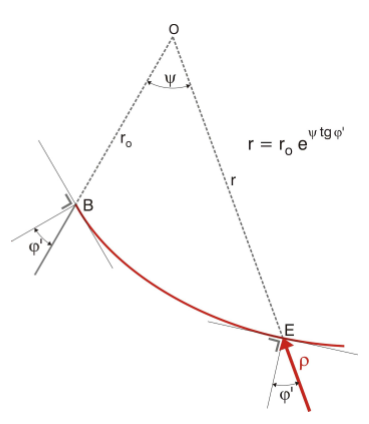
\includegraphics[scale=0.6]{Holeyman/images/H22.PNG}
                \caption{Définition d’une spirale logarithmique }
                \end{figure}
                
            \end{multicols}
            
            \textit{"Cette spirale à pour caractéristique que la normale en tout point forme un angle $\phi'$ avec le rayon vecteur passant par ce point. Dès lors, une contrainte agissant sur une facette tangente à la spirale logarithmique passera par le pôle de la spirale si son obliquité (par rapport à la normale) est de $\tan \phi$. Cette condition correspond exactement à la mobilisation de la résistance ultime en cisaillement du sol selon le critère de Mohr-Coulomb pour $c=0$."}
            
            J'ai pas tout compris à la démonstration, elle est trouvable entre les pages 13 et 15 du PDF "fondation superficielles 2015".
            
            En fin de démonstration, on trouve une expression du pouvoir portant $q_ult$ sous une forme canonique similaire à la précédente sans le terme $N_{\gamma}$ puisque dans les hypothèse, le sol est supposé sans poids propre.
            
            \begin{center}
                \begin{tabular}{c|c}
                     $q_{ult} = c N_c + q N_q$ &  $N_c = (N_q - 1) \cot \phi$ \\   
                \end{tabular}
            \end{center} 
            
            \underline{Formule de Buisman:} 
            
            Buisman complète la formule de Prantl en y introduisant le terme de portance relatif au poids propre. Il prend l'hypothèse (sur base d'observation) de conserver la forme de rupture de Prandtl et d'y ajouter le poids propre du sol (En somme il enlève juste une hypothèse parce qu'il a pas envie de se fouler !) On obtient alors une nouvelle formule:
            
            \begin{center}
                $q_{ult} = c N_c + q N_q + \frac{1}{2} \gamma N_{\gamma} B$
            \end{center}
            
            Il existe des tableaux qui reprennent les courbes de Prandtl-Buisman qui nous donne les valeurs numériques des trois coefficients en fonction de la cohésion. Mais pour le principe, voici les formules pour les calculer:
            
            \begin{center}
                $N_q = e^{\pi \tan \phi} \tan^2(\frac{\pi}{4} + \frac{\phi}{2})$ 
                \medskip
                $N_c = (N_q - 1) \cot \phi$ 
                \medskip
                $\frac{1}{2} N_{\gamma} = \frac{1}{8}[\frac{1+K_p}{1+9 \tan^2 \phi} \{(3\tan \phi \sqrt{K_p}-1) e^{\frac{3\pi}{2} \tan \phi} + 3 \tan \phi \sqrt{K_p} \} + 2K_p e^{\frac{3\pi}{2} \tan \phi} - 2 \sqrt{K_p}]$
            \end{center}
            
        \subsubsection{Théorie de Terzaghi}
        
            Cette théorie se base en grande partie sur les hypothèses introduites dans la théorie de Prandtl. 
            
            Hypothèses : \begin{itemize}
                \item problème bidimensionnel
                \item fondation rugueuse
                \item l'angle supposé par Prandtl devient $\phi$ plutôt que $(\frac{\pi}{4} + \frac{\phi}{2})$. L'angle de la spirale logarithmique devient donc $(\frac{3\pi}{4} - \frac{\phi}{2})$
                \item la fondation est enterré à une profondeur D, on a donc une surcharge verticale à la surface du massif $q=\gamma D$ (la résistance au cisaillement du sol au-dessus des fondations est négligé)
            \end{itemize} 
            
            les valeurs obtenues par Terzaghi sont:
            \begin{itemize}
                \item terme de \textbf{Profondeur}: $N_q = \frac{a^2}{2 \cos^2(\frac{\pi}{4} + \frac{\phi}{2})}$
                \item terme de \textbf{Cohésion}: $N_c = \cot \phi (\frac{a^2}{2 \cos^2(\frac{\pi}{4} + \frac{\phi}{2})}-1)$
                \item terme de \textbf{Surface}: $N_{\gamma} = 2 \tan \phi (N_q + 1)$
            \end{itemize}
            
            \begin{center}
            avec $ a = e^{(\frac{3\pi}{4} - \frac{\phi}{2}) \tan \phi}$ 
            \end{center}
            
            En pratique on utilise des tables de valeurs pour ces trois coefficients.
            
    \subsection{Charge inclinée excentrée: Méthode de Vesic et de Hansen}
        
        \subsubsection{Formule généralisée du pouvoir portant}
        
            Les hypothèses des théories mentionnées ci-dessus sont toujours trop restrictives pour pouvoir être appliquée dans un cas pratique. De Beer, Hansen et Vesi ont rajouté un paqut de coefficient pour corriger les méthodes précédentes en compte de la profondeur, la forme de la fondation, l'inclinaison et la charge. En gros c'est pas bien différent de ce qu'il ont fait au-dessus, les résultats sont très proche mais c'est mieux ! On a donc une nouvelle forme canonique:
            
            \begin{center}
                \begin{tabular}{c|c}
                    $q_{ult} = s_c d_c i_c c N_c + s_q d_q i_q q N_q + \frac{1}{2} \gamma s_{\gamma} d_{\gamma} i_{\gamma} N_{\gamma} B$  
                        &   s: (Shape) dépend de la forme \\
                        &   d: (Depth) dépend de la profondeur \\
                        &   i: (Inclinaison) je te laisse deviner 
                \end{tabular}
            \end{center}
            
            \underline{Prise en compte de la profondeur de la fondation:} 
        
            Pour le pouvoir portant, il faut tenir compte du fait que la fondation est enterrée. On ne peut négliger la résistance au cisaillement de la couche situé au-dessus du niveau de la fondation. Par ailleurs on suppose que la forme de la surface de rupture n'est pas influencé par cette résistance superficielle, alors que le mécanisme de rupture devrait respecter le principe "de la recherche d'énergie minimum". 
            
            \begin{figure}[h!]
                \centering
                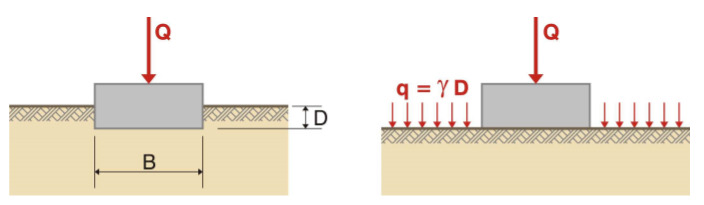
\includegraphics[scale=0.8]{Holeyman/images/H23.PNG}
                \caption{Considération de la profondeur de la fondation selon l’équation canonique }
            \end{figure}
            
            La valeur des coefficients généralement proposées en fonction de la profondeur $D$ et de la base $B$ de la fondation sont données dans des tableaux. (Trouvable page 20-21 du PDF "fondation superficielles 2015"). 
            
            \underline{Prise en compter de la forme de la fondation:} 
        
            Dans les résolutions précédentes on se réfère à des problèmes bidimensionnels (semelle filante), c'est à dire un rapport longueur / largeur très grand. Cette estimation est bonne si ce rapport est supérieur à 8. En pratique on l'accepte pour un rapport supérieur à 5 (après tout hein !). Dans le cas contrainre, la surface de rupture à un caractère tridimensionnel marqué dont il faut tenir compte. Cela aura pour effet d'augmenter les contributions de $N_c$ et $N_q$ et de diminuer la contribution du poids propre du sol qu'elle englobe (donc diminuer $N_{\gamma}$) car la rupture cherche à déployer un minimum d'énergi . les différentes valeurs sont à nouveau reprises dans des tableaux. (Trouvable page 21-22 du PDF "fondations superficielles 2015"). 
            
            \underline{Prise en compte de l'inclinaison de la sollicitation:} 
            
            Souvent le cas lors de la construction de fondation d'arcs ou de portique mais aussi pour des constructions ou les forces dues au vent se cumulent à la gravité. Finalement on retrouve ce type de sollicitation dans des structures reprenant des efforts de freinage ou de roulement.
            
            La surface de rupture n'est plus symétrique mais développé dans la direction de la charge. On a donc une réduction du pouvoir portant par rapport au cas d'une fondation supportant uniquement une charge verticale (Tableaux page 23-24). 
            
            \underline{Prise en compte de l'excentricité de la sollicitation:} 
            
            On trouve ce genre de situation lorsque l'emprise de la fondation est restreinte par la proximité d'un obstacle ou par une limite de propriété. C'est aussi le cas d'une fondation existante qui recevait une charge centré et qui perd une partie de se surface portante lors de transformation, rénovation,... C'est également toujours le cas pour la fondation d'une éolienne, la force du vent entraîne un bras de levier qui décentre la charge sur la fondation.
            
            Plutôt que de résoudre un problème se compliquant avec un distribution de contrainte très contrasté, qui met rapidement en défaut l'hypothèse de faibles déformations (voir p26) la pratique consiste à calculer le pouvoir portant sur base d'une répartition uniforme, centrée sur la force appliquée. Cela revient à ne considérer comme largeur $B'$ de la fondation la partie de la fondation centrée sur la force.
            
            Dans le cas d'une double excentricité, on ne tient compte que de la partie de la fondation centrée sur l'axe de la sollicitation. On base donc le calcul sur des dimensions $B'$ et $L'$ réduites.
            
            \begin{multicols}{2}
            
                \begin{figure}[h!]
                \center
                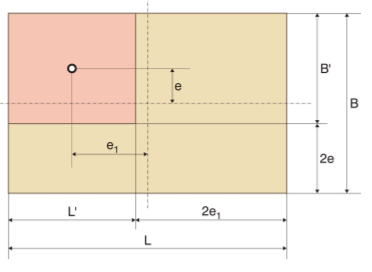
\includegraphics[scale=0.8]{Holeyman/images/H24.PNG}
                \caption{Double excentricité}
                \end{figure}
            
            \vfill\null\columnbreak
            
                \begin{figure}[h!]
                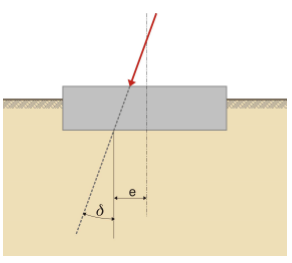
\includegraphics[scale=0.8]{Holeyman/images/H25.PNG}
                \caption{ Séparation de l’inclinaison et de l’excentricité de la charge}
                \end{figure}
                
            \end{multicols}
            
            \begin{center}
                \begin{tabular}{cc}
                     $B' = B - 2e$ \: \: \: &  $L' = L - 2e_1$   
                \end{tabular}
            \end{center} 
            
            Il s'en suit d'une surface de calcul $A' = B'L'$ et une charge ultime $Q_{ult} = q_{ult} B' L'$. On remarque qu'une charge inclinée va souvent de pair avec l'application d'une excentricité. Il faut analyser séparément l'effet de l'inclinaison et de l'excentricité.
            
    \subsection{Tassement des fondations superficielles}
    
        Il est essentiel de pouvoir estimer l'état des contraintes qui apparaissent lorsque le sol est sollicité par une charge extérieur. La contrainte verticale qui s'exerce sur un plan horizontal se divise en deux parties. Une première, uniforme, est due au poids des couches de sols. La seconde est l'incrément de contrainte dû à la surcharge (courbe de gauss centrée au point d'application).
        
        Chaque grain se repose sur ceux en dessous qui à leur tour se reposent sur ceux d'en dessous,... La charge entraîne donc une contrainte qui a tendance à se répartir avec la profondeur (à la manière d'un phénomène de diffusion).
            
            \subsubsection{Approche simplifiée}
            
            Considérons le problème en deux dimensions. On sépare notre fondation en un empilement de rouleau supportant une charge locale (3D en un ensemble de sphère). On simplifie le problème en considérant que la contrainte provoquée par la surcharge ponctuelle soit uniformément répartie sur une surface délimitée par un cône d'ouverture $2\beta$. 
            
            \begin{multicols}{2}
            
                \begin{figure}[h!]
                \center
                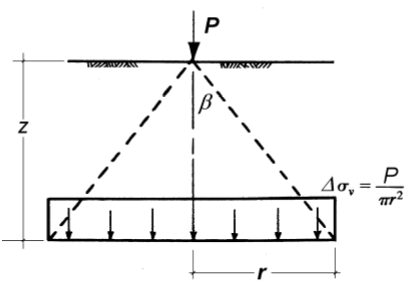
\includegraphics[scale=0.6]{Holeyman/images/H26.PNG}
                \end{figure}
            
            \vfill\null\columnbreak
            
                \begin{figure}[h!]
                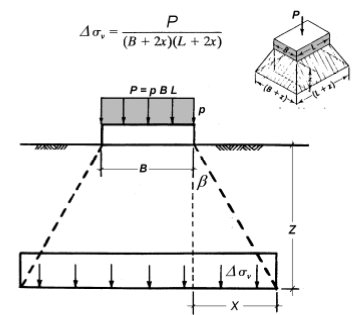
\includegraphics[scale=0.6]{Holeyman/images/H27.PNG}
                \end{figure}
                
            \end{multicols}
            
            On peut facilement estimer la contrainte répartie sur cette nouvelle surface: 
            
            \begin{center}
            \begin{tabular}{c|c}
                $\sigma_z = \rho \frac{BL}{(B+2x)(L+2x)}$ \: \: &  $ x = z \tan(\beta) $ 
            \end{tabular}
            \end{center} 
            
            En pratique, les valeurs de $\beta$ les plus souvent utilisées sont:
            
            \begin{center}
            \begin{tabular}{ccc}
                 $\beta = \frac{\pi}{4}-\frac{\phi}{2}$ & $30°$ & $\tan \beta = \frac{1}{2}$  
            \end{tabular}
            \end{center} 
            
            L'hypothèse de base est fausse, les valeurs obtenues avec ces évaluations sont donc erronées mais permettent d'avoir rapidement un premier ordre de grandeur. On considère qu'une charge ponctuelle provoquerait une contrainte de profondeur uniformément répartie. Hors, il suffit de diviser la base en plusieurs rectangle et d'appliquer cette approche simplifié sur chacun d'entre eux pour s'apercevoir que la contrainte de profondeur aura plus l'allure d'une courbe de Gauss.
            
            \subsubsection{Charge verticale ponctuelle}
            
            \underline{Loi de Boussinesq:} 
            
            Hypothèse sur le massif:
            \begin{itemize}
                \item semi-infini
                \item élastique (caractéristiques: E module élasticité et $\nu$ coéficient de poisson)
                \item homogène (E et $\nu$ constant en tout point du domaine)
                \item isotrope (E et $\nu$ ne dépendent pas de la direction)
            \end{itemize} 
            
            Hypothèse sur la charge$P$:
            \begin{itemize}
                \item ponctuelle
                \item perpendiculaire au plan limitant le demi-espace
            \end{itemize} 
            
            La loi de Boussinesq donne le champ de contrainte en tout point de coordonnées polaires $(r, \theta)$ vis à vis du point d'application de la force en surface.
            
            \begin{center}
                $\sigma_z = \cos^3 \theta \frac{3 P}{2 \pi r^2} = \frac{3 P z^3}{4 \pi r^5} = \cos^5 \theta \frac{3 P}{2 \pi z^2}$
            \end{center} 
            
            Le champ de déplacement vertical $w$ du massif est donné par:
            
            \begin{center}
                $w = P \frac{1+\nu}{2 \pi E r} (\cos^2 \theta + 2(1-\nu))$
            \end{center} 
            
            On observe que $w$ tend vers l'infini lorsque r tend vers 0 et qu'il devient nul lorsque $r$ tend vers l'infini (pour des $\nu$ admissible).
            
            Ce modèle est critiquable, le sol n'est ni linéaire ni isotrope et l'homogénéité mécanique du massif n'est pas justifiable. On a vu que le module de déformation d'un milieu granulaire croit avec la contrainte initiall de référence. Il est donc plus indiqué de modéliser le comportement du sol par un module croissant avec la profondeur (ex: $E_{oed}$).
            
            Cependant la valeur de $\sigma_z$ ne dépend pas du module d'élasticité $E$. Cette équation est donc couramment utilisée dans les calculs de tassement de fondations.
            
            \underline{Loi de Fröhlich:}
            
            Elle s'inspire de Boussinesq mais est plus générale. Il a modifié les équations en y introduisant un paramètre $\lambda$ appelé \textit{paramètre de concentration de contraintes} ou \textit{indice de Fröhlich}. L'apport de contrainte vertical change d'équation:
            
            \begin{center}
                $\sigma_z = \frac{\lambda P}{2 \pi z^2} \cos^{\lambda +2} \theta $
            \end{center} 
            
            L'indice de Fröhlich varie de 1 à 6 suivant l'équation:
            
            \begin{center}
                $\phi(\lambda, \theta) = \frac{1}{2} \lambda \cos^{\lambda+2} \theta$
            \end{center} 
            
            On retrouve les différentes courbes obtenues dans les diagrammes.
            
            \underline{Loi de Buismann:} 
            
            Hypothèse:
            \begin{itemize}
                \item sol incompressible ($\nu = \frac{1}{2}$) (mais déformable, $E$ et $G$ sont défini)
                \item module d'élasticité varie linéairement ($E = \beta z$) avec la profondeur
                \item sol orthotrope et $E_h$ (horizontal) conserve un rapport constant avec $E_v$ (vertical) $n=cst=\frac{E_h}{E_v}$
                \item le module d'élasticité $E_{\theta}$ (direction quelconque) se déduit de la rotation des axes, il est donné par: $E_{\theta} = E_v \cos^2 \theta + E_h \sin^2 \theta$
            \end{itemize}
            
            Dans la loi de Buismann (équation ci-dessous), la valeur de $\sigma_z$ ne dépend pas de $\beta$ (Cette observation est analogue à l'indépendance de l'équation de Boussinesq vis-à-vis de $E$ et $\nu$).
            
            \begin{center}
                $\sigma_z = \frac{6P}{(n+2) \pi z^2} \cos^6 \theta (\cos^2 \theta + n \sin^2 \theta)$
            \end{center} 
            
            \underline{Comparaison des trois lois:} 
            
            Comparons les valeurs obtenues avec une charge $P$ d'inclinaison nulle ($\theta = 0$).
            
            L'équation de Fröhlich et celle de Buisman s'identifie pour $\lambda = \frac{12}{n+2}$.
            
            \begin{itemize}
                \item $\lambda = 1 \to n=10 $
                \item $\lambda = 2 \to n=4 $
                \item etc.
            \end{itemize} 
            
            Rappel: le rapport des contraintes horizontales et verticales en un point est compris entre deux limites ($K_a$ l'état passif et $K_p$ l'état actif). 
            
            Si l'on souhaite que le rapport $\frac{E_h}{E_v}$ s'apparente au rapport $\frac{\sigma_h}{\sigma_v}$, on constate que seul les $n$ compris entre 0.4 et 4 ($\to \lambda = 2$ ou $5$) sont acceptables.
            
            En europe on utilise $\lambda = 3$ ou $4$.
            \begin{itemize}
                \item $\lambda = 3$ correspond à deux cas:
                \begin{itemize}
                    \item matériaux qui obéit à la loi de hooke dans un milieu homogène, élastique et isotrope avec un coefficient de poissont $\nu = \frac{1}{2}$ (hypothèse de Boussinesq). Correspond à un sol argileux saturé (Typique anglo-saxon)
                    \item matériaux qui obéit à la loi de Buisman avec $E_h = 2E_v$
                \end{itemize}
                \item $\lambda = 4$ correspond à l'hypothèse de Buismann ($E=\beta z$) module d'élasticité isotrop et $\nu=\frac{1}{3}$. Il s'agit d'un sol sableux, typiquement belge, hollandais, ...
            \end{itemize}
            On analyse au cas par cas quelle hypothèse utiliser.
            
            \subsubsection{Fondation de forme régulière ou quelconque}
            
            Il est possible d'obtenir les contraintes dans un massif semi-infini élastique soumis à une charge non ponctuelle. On divise la zone chargée en sections élémentaires que l'on considère chargées ponctuellement en leur centre et on somme les effets obtenus. Moyennant la validité du principe de superposition, des solutions existent pour des surfaces simples chargées uniformément ou linéairement. Pour des situations plus complexes des solutions sont obtenues grâce à l'informatique et aux méthodes numérique. 
            
            \underline{Validité du principe de superposition:} 
            
            Ce principe est applicable de manière générale si les déformation sont proportionnelles aux contraintes: $\sigma = E \epsilon$
            
            Il est également applicable si le sol est hétérogène et anisotrope SSI:
            \begin{itemize}
                \item $\sigma = E \epsilon$ en tout point (les coefficients pouvant varier)
                \item les coefficients doivent être les même dans le plan horizontal pour une même direction
            \end{itemize} 
            Et si le sol ne répond pas vraiment à ces conditions (mais bon faut bien faire quelque chose), on peut l'appliquer si:
            \begin{itemize}
                \item la modification de contrainte soit relativement faible par rapport à l'initial
                \item pour tout point d'un même plan horizontal les modifications sont de même signe
            \end{itemize}
            L'étude des diagrammes expérimentaux de mise en charge de fondations montre qu'en pratique il existe un domaine de comportement linéaire pour lequel le principe de superposition peut être appliqué. Il donne des résultats suffisamment proche de la réalité.
        
            
                \underline{Steinbrenner-Fadum: rectangle chargé uniformément}
            
                Cette solution intègre la formule de Boussinesq pour une charge rectangulaire (une charge uniformément répartie est une infinité de charges ponctuelles).
            
                \begin{figure}[h!]
                    \centering
                    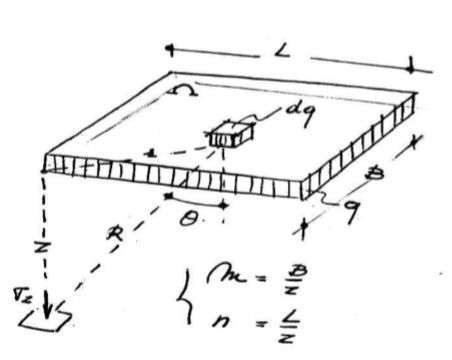
\includegraphics[scale=0.8]{Holeyman/images/H28.PNG}
                    \caption{Semelle rectangulaire uniformément chargée}
                \end{figure}
            
            On considère un rectangle élémentaire $dA = dX dY$ chargé par une charge élémentaire $dq$. On prend la formule de Boussinesq avec $r=R$, $P=dq$ et $\sigma_z = d\sigma_z$. On l'intègre sur la surface $\Omega = B L$.
            
            Changement de variable car $dq = q dX dY$. On développe et on obtient:
            
            \begin{center}
            \begin{tabular}{c|c|c}
                 $\sigma_z = q K$ \: \: \: &  $K=\frac{1}{2} \pi (\frac{mn}{s} (\frac{1}{M}+\frac{1}{N}) + \arctan \frac{mn}{S})$ 
                    &   $M = 1+m^2$  et  $m = \frac{B}{z}$ \\
                  & &  $N = 1+n^2$  et  $n = \frac{L}{z}$ \\
                  & &  $S = \sqrt{1+m^2+n^2}$  \\
            \end{tabular}
            \end{center}
            
            Le coefficient d'influence $K$ est donné en diagramme lors des exercices.
            
            Il est important de remarquer que la formule fournit une valeur de la contrainte verticale $\sigma_z$ sous le coin de la fondation (d'où le fait que $K$ tende vers $\frac{1}{4}$ pour $z = 0$). Dans le cas où la charge n'est pas sur le coin, il faut diviser la fondation en plusieurs sous partie et composer avec celles-ci pour obtenir la valeur de la grande. 
        
            
                \underline{Newmark: fonction circulaire uniformément chargée} 
            
                Pareil que précédemment mais on intègre sur un cercle. On ne s'occupe que du cas ou la charge est centrée (une solution plus générale existe mais n'est pas développé).
            
                \begin{figure}[h!]
                    \center
                    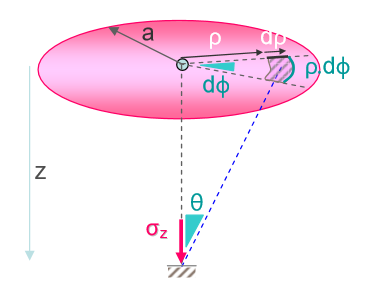
\includegraphics[scale=0.8]{Holeyman/images/H29.PNG}
                    \caption{Contraintes verticales sous le centre d'une fondation circulaire uniformément chargée}
                \end{figure}
            
            On passe coordonnées cylindrique ($p, \phi, z$), on considère une portion du cercle $d\omega$ chargée par une chrge $dq$. On intègre simplement sur la surface en faisant un changement de variable $dq = q d\omega = q p d\phi dq$ et en remarquant que $R^2 = p^2 + z^2$. On obtient:
            
            \begin{center}
            \begin{tabular}{c|c}
                 $\sigma_z = q K$ \: \: & $K = 1-(\frac{1}{1+(\frac{a}{z})^2})^{\frac{3}{2}} $
            \end{tabular}
            \end{center} 
            
            $K$ est le coefficient d'influence de Newmark (adimensionnel). Il caractérise l'influence à la profondeur $z$ d'une charge uniformément répartie sur un cercle de rayon $a$. Il existe un abaque sous forme de rosace qui permet de calculer $K$ pour une fondation quelconque (Mode d'emploi de cet abaque à la page 42 du PDF sur les fondations superficielles).
            
            \underline{Fondation triangulaire uniformément chargée:}
            
            Il est possible d'intégrer n'importe quelle forme de fondation grâce à des programmes informatiques. Le programme divise la surface en un maillage généralement carré ou triangulaire. Reste donc à savoir intégrer sur une forme triangulaire (temps de se remettre au C).
            
            On prend un élément triangulaire supportant une charge q uniforme. On applique Boussinesq et le principe de superposition, il faut donc intégrer sur la surface. On fait un changement de variable $dq = q d\omega = q dq p d\phi$
            
            On intègre la surface du triangle pour un angle $\phi$ avec p qui varie de 0 à $\frac{a}{\cos \phi}$ avec $\phi$ compris entre 0 et $\phi_b = \arctan \frac{b}{a}$ 
            
            On obtient:
            
            \begin{center}
            \begin{tabular}{c|c}
                $\sigma_z = \frac{q}{2 \pi}(\arctan \frac{\beta}{\alpha}-\arctan\frac{\beta}{\alpha+ \sqrt{1+\alpha^2\beta^2}}+\frac{\alpha\beta}{(1+\alpha^2)\sqrt{1+\alpha^2\beta^2}})$ \: \:
                    &  $\alpha = \frac{a}{z}$ [rad] \\
                    &  $\beta = \frac{b}{z}$ [rad]  
            \end{tabular}
            \end{center} 
            
            Cette formule n'est valable que sous l'angle droit d'un triangle. Si le triangle n'est pas rectangle, il faut le diviser en plus petit triangle rectangle. Pour un maillage en carré, il faut que la charge soit centrée et le résultat ne sera acceptable qu'à partir d'une profondeur d'environ trois fois la taille de la maille. Contrainte excessive pour une profondeur inférieur voir infinie pour $z=0$ (les triangle c'est mieux que les carrés !).
            
            \subsubsection{Le bulbe d'influence}
            
            Quand on applique une charge sur une fondation, la contrainte dans le sol ne décroît pas linéairement avec la profondeur. Pour voir l'évolution de cette contrainte, il faut dessiner le diagramme \textit{d'iso-contraintes} ou \textit{diagramme isobare des contraintes}. Dans la littérature ce diagramme est appelé \textit{bulbe des contraintes} de par sa forme (dans le cas d'une semelle filante uniformément chargée).
            
            \begin{figure}[h!]
                \centering
                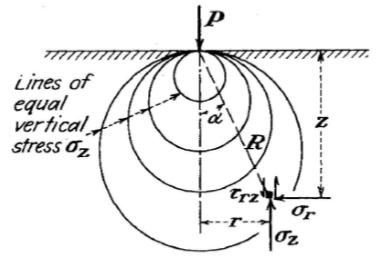
\includegraphics[scale=0.8]{Holeyman/images/H30.PNG}
            \end{figure}
             
            \underline{Effet d'échelle: } 
            
            La profondeur d'influence d'une charge est proportionnelle à la dimension transversale de celle-ci. On peut observer cela grâce à la formule de Newmark et à l'étude de son coefficient d'influence K. On peut raisonnablement considérer que la fondation n'a plus d'influence lorsque $K$ est inférieur ou égale à 0.1. Dans le cas de Newmark pour $\frac{a}{z} = 0.27$ vu que  $a$ est le rayon et $B$ le diamètre, on peut avec des maths super compliqué trouver que $z \approx 2B$ pour que ce rapport soit vérifier. On a une zone d'influence pour une surface circulaire de $2B$ soit deux fois le diamètre.
            
            Si le sol est homogène, la fondation de plus grande taille apportant la même pression de contact $p$ subit un tassement plus grand puisque chaque couche de sol quel que soit sa profondeur subit un accroissement de contraintes. Dans le cas d'un sol hétérogène, c'est encore plus marqué. Une couche incompressible profonde pourrait ne pas être influencée par une fondation étroite alors qu'une large l'influencerai significativement (d'où une différence de tassement importante entre ces deux géométries).
            
            On peut l'appliquer sur une semelle carré (pareil $z \approx 2B$). Par contre une semelle rectangulaire filante de largeur B produit un plus grand effet (logique, alignement du carré à l'infini pour former une semelle filante rectangulaire $\to$ addition de tous les bulbes $\to$ plus grande contrainte). On constate que $z \approx 6B$ pour un coefficient d'influence de 0.1. 
            
            \begin{figure}[h!]
            
            \underline{Effet de proximité et de juxtaposition: } 
            
            On comprend intuitivement que si l'on place deux fonctions proches l'une de l'autre, la zone comprise dans la zone d'influence des deux fondations subira plus de contraintes. 
            
                \centering
                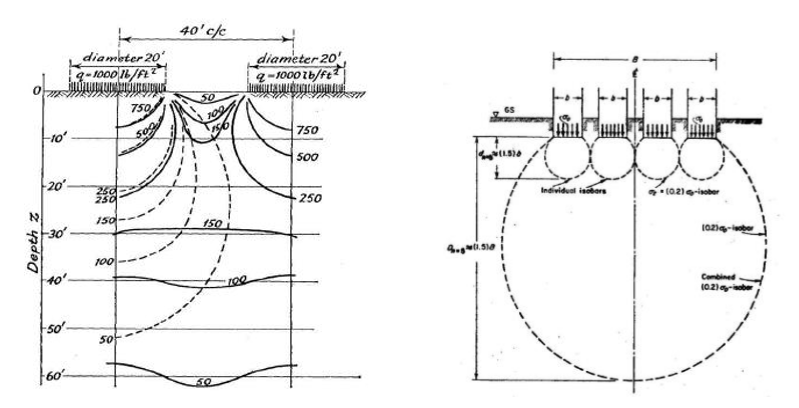
\includegraphics[scale=0.8]{Holeyman/images/H31.PNG}
            \end{figure}
            
            Le bulbe de contrainte en pointillé représente l'influence d'une fondation isolée, les courbes en traits pleins représentent la juxtaposition. On remarque peut de différence sous la fondation mais les contraintes sont non négligeable dans l'intervalle inter-fondation; Les courbes profondes se réunissent pour englober l'effet des deux fondations et n'en former qu'une. le schéma de droite montre le phénomène d'échelle, la division en plusieurs petites fondations permet de limiter la zone d'influence générale. 
            
            \subsubsection{Calcul du tassement}
            
            \underline{Méthode graphique:} 
            
            La compression $ds$ d'une couche de sol de hauteur $dh$ lorsque la contrainte effective augmente de $\sigma_z \to \sigma_z + \Delta \sigma_z$ s'exprime par la loi de Terzaghi:
            
            \begin{center}
            \begin{tabular}{c|c}
                $ds = \frac{dh}{C} \ln \frac{\sigma_z + \Delta \sigma_z}{\sigma_z}$ 
                    &  C: constante de compressibilité  \\
                    &  $\sigma_z$: contrainte naturelle effective  
            \end{tabular}
            \end{center}
            
            On intègre cette expression sur l'épaisseur de sol situé sous le niveau de fondation. On peut ensuite tracer un graphique logarithmique ($E_{log} - E_h$). Ou l'on peut remplacer les vrai grandeurs par leur représentation à l'échelle: $h=h E_h$ et $\ln = \ln E_h$
            La constante de compressibilité peut être considérée comme constante pour une couche déterminée de sol. On peut remplacer $C$ par une somme de constante pour $n$ couche $i$ caractérisée par $C_i$. On résout l'équation et l'expression du tassement s'écrit:
            
            \begin{center}
                $s = \frac{1}{\bar{E_h}\bar{E_{ln}}} \sum_{i=1}^{n}\frac{\bar{S_i}}{C_i}$
            \end{center}
            
            Le tassement ainsi calculé représente le tassement à l'équilibre final. Il faut prendre en compte le phénomène de consolidation pour évaluer à quel rythme le tassement va se produire, spécialement pour des sols fins saturés.
            
            \underline{Composantes du tassement:} 
            
            La tassement total se divise en trois composantes:
            \begin{itemize}
                \item Tassement vertical
                \item Rotation d'ensemble
                \item Distorsion (nuisible car déforme et donc sollicite la structure)
            \end{itemize} 
            
            \underline{Le tassement différentiel:} 
            
            Il s'exprime entre deux appuis voisins d'une même structure ou le tassement est différent. Il induit une distorsion de la structure (d'angle $\alpha$).
            
            \begin{figure}[h!]
                \centering
                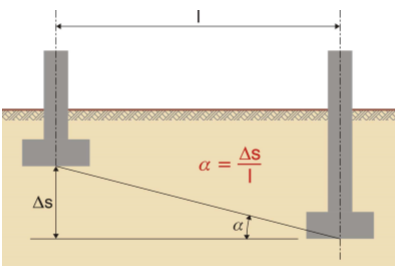
\includegraphics[scale=0.8]{Holeyman/images/H32.PNG}
                \caption{Tassement différentiel}
            \end{figure}
            
            Il n'est dans l'absolu pas possible de définir une valeur de tassement admissible. On peut estimer une borne supérieur qui mènerait à la ruine de la structure, mais elle n'est pas suffisamment restrictive. Tout dimensionnement requiert une double vérification (ELU et ELS). La seconde vérification concerne les fonctionnalités de l'ouvrage qui peuvent être mise à mal par une structure trop déformée. Le tassement admissible dépend donc des conséquences considérées comme admissibles. Par exemple, on peut fixer une limite en fonction des matériaux utilisés de manière à éviter l'apparition de fissure.
            
            Un tassement différentiel peut s'exprimer au sein de l'ouvrage mais aussi dans une semelle ou un radier. de comportement intermédiaire sont possible:
            \begin{itemize}
                \item la semelle est souple (ex: tôle en acier,...) et la distribution de contraintes correspond à une pression uniforme exprimée en fonction de la charge en présence. Le tassement est plus élevé au centre que sur les bords (en accord avec le bulbe d'influence).
                \item la semelle est rigide et la distribution de contrainte uniforme. Les contraintes en périphérie seront plus importante qu'au milieu pour produire un tassement uniforme.
            \end{itemize}
            
            En pratique, la semelle affecte une raideur intermédiaire tendant à produire une courbure concave. La contrainte de contact entre la fondation et le sol dépend donc de la raideur de la fondation. Il est possible de calculer la cuvette de tassement de semelle. Dans la pratique, on contourne le problème en utilisant la notion de point singulier (point ou le tassement est indépendant de l'hypothèse de raideur établie pour répartir les pressions de contacts). 
            
            \begin{figure}[h!]
            \underline{Les causes du tassement défférentiel:}
            
            \begin{itemize}
                \item Sous sol hétérogène: (ex: tou de Pise) le tassement est plus grand là ou le sol est plus compressible.
                 \item Fondation hétérogène: la partie la moins profonde risque de plus tasser que l'autre, fissurant ou rompant l'interface des deux parties.
                 \item Charges non uniformes: la partie la plus chargée se tassera si toutes les fondations sont identiques.
                 \item Fondations à niveau différents ($\approx$ fondation hétérogène)
                 \item Présence de points durs: lorsqu'une fondation homogène est établie sur un point dur (ex: ancienne fondation, égouts,...)
                 \item Remblai partiel: une zone remblayée tasse d'avantage.
                 \item Bâtiments d'âge différents: la construction d'un nouvel ouvrage vient ajouter des contraintes sur le sol d'un ouvrage existant.
                 \item Raideur de la fondation: fondation souple entraine une contrainte uniforme et un tassement non uniforme.
                 \item Rabattement de la nappe: si la nappe est rabattue, cela diminue les contraintes effective, il y a donc un plus grand tassement dans une zone ou une nappe a été rabattue (Rabattement par pompage, par la végétation, par une fouille).
                 \item Gonflement hydrique: gonflement du sol lorsque la construction est établie à une profondeur insuffisante.
                 \item Assèchement et retrait: le sol réduit le volume par assèchement, une fois à la limite de retrait il va craqueler, si les fondations ne sont pas assez grande, il y aura fissuration.
                 \item Arbres et sols plastiques: si une des fondations est dans la zone d'influence des racines d'un arbre a croissance rapide.
                 \item Interactions entre bulbes de contraintes ($\approx$ Bâtiments d'âges différents).
            \end{itemize}
            
            Une des solutions pour contrer le tassement différentiel est le \textbf{chaînage horizontal} des murs porteurs (armatures qui reprennent les efforts en tractions).
            \end{figure}
            
            
\section{Fondations profondes}
    
    Ce type de fondation est utilisé lorsque le pouvoir portant du sol est insuffisant à faible profondeur ou que les tassements absolus ou différentiels ne sont pas compatibles. Le type de fondation profonde le plus courant est la fondation sur pieu généralement prismatique (souvent cylindrique). Ils transmettent la charge qu'ils reçoivent en tête vers les couches de sol en profondeur.
    
    \subsection{Généralités}
    
        \subsubsection{Mode de portance d'un pieu}
        
        Deux principaux modes de fonctionnement:
        \begin{itemize}
            \item résistance à la base: on rencontre dans une profondeur économiquement atteignable une couche de sol très résistante ou l'on va s'ancrer.
            \item flottante: il n'y a pas à proximité de couche plus résistante, on doit donc se reposer sur les forces de frottement latérales dans des couches à résistance moyenne.
        \end{itemize} 
        
        On retrouve généralement une combinaison de ces deux effets. La charge limite pouvant être appliquée en tête de pieu est donc la somme de la charge limite pouvant être supportée en base et la charge reprise par frottement: $Q_t = Q_b + Q_s$ 
        
        Afin d'augmenter ce pouvoir portant, on élargi la base.
        
        \begin{figure}[h!]
            \centering
            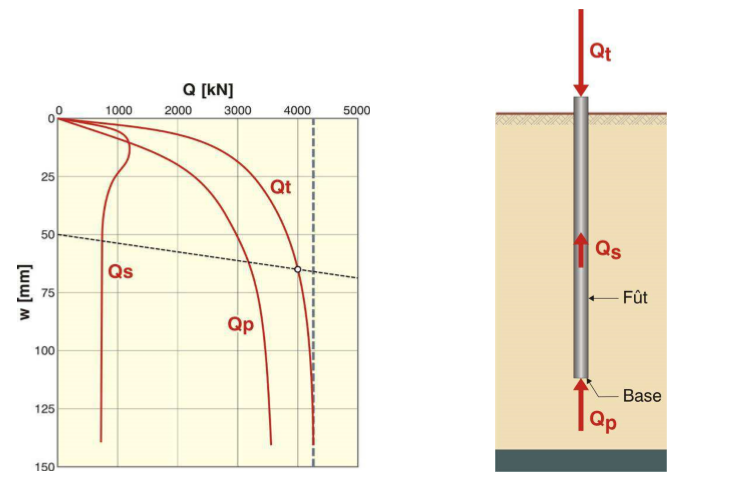
\includegraphics[scale=0.8]{Holeyman/images/H33}
            \caption{Courbes de mobilisation de la réaction du sol}
        \end{figure}
        
        \subsubsection{Essai de mise en charge statique}
        
        Cet essai vise à caractérisé l'aptitude de la fondation à reprendre des charges importantes sans subir des tassements excessifs. On applique progressivement (par palier) une très grande charge sur un pieu préalablement enfoncé dans le sol (grâce à des vérins et des ballasts) et on mesure le tassement en tête de pieu. On détermine ainsi sa charge limite en le poussant à la rupture (vérifie aussi que les déformations sont acceptables).
        
        Il faut bien évidemment dimensionner le pieu pour éviter toute rupture organique de ses matériaux constituants, fautes de quoi les résultats seraient faussés.
        
        Le tassement total du pieu est la somme du tassement à la base du pieu et du raccourcissement élastique du fût. Afin de bien les distinguer, des extensomètre sont placés à l'intérieur du fût à intervalles réguliers. On obtient la déformation unitaire du pieu.
        
        \begin{center}
        \begin{tabular}{cc}
            $\epsilon = \frac{\Delta L}{L}  $  & microstrain [$\mu str = 10^{-6}$]
        \end{tabular}
        \end{center} 
        
        \begin{figure}[h!]
            \centering
            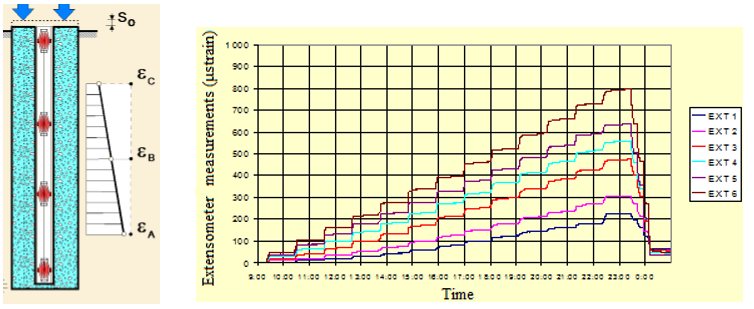
\includegraphics[scale=0.8]{Holeyman/images/H34.PNG}
            \caption{Mesures extensométriques:  (a) configuration dans le pieu  (b) mesures en fonction du temps}
        \end{figure}
        
        On consrate une grande différence entre le raccourcissement unitaire entre la tête du pieu (Ext6) et la base (Ext1). On remarque que les efforts sont plus grand en tête qu'en base de pieu. C'est du aux forces de frottement. On est dans le cas d'une déformation élastique qui s'exprime selon la relation suivante: 
        
        \begin{center}
        \begin{tabular}{c|c}
            $F = EA \epsilon$  & EA: module de raideur [KN] (section du pieu \& module de young) 
        \end{tabular}
        \end{center} 
        
    \subsection{Type de pieu}
    
        \subsubsection{Classification des pieux}
        
        Il sont mis en place suivant deux procédés extrème:
        
        \begin{itemize}
            \item Pieu mis en place par refoulement: Le sol est totalement refoulé et donc essentiellement mit en compression, la composante latérale induit un état limite passif (mise en butée).
            \item Pieu mis en place par excavation du sol: Le sol est généralement décomprimé, la contrainte géostatique horizontale préexistante est réduite et évolue vers un état limite actif (poussée).
        \end{itemize} 
        
        Les pieux à refoulement sont préfabriqué (en bois, béton armé/précontraint ou en acier). Ils sont mis en place par battage, vérinage, vissage ou vibration. On y trouver aussi les pieds moulé dans le sol à condition qu'ils soient mis en place de telle sorte qu'à aucun moment le terrain ne soit décomprimé.
        
        Les pieux mis en place par extraction sont constitué de béton armée, non armé ou mixte. En somme, on retient la terre, on met le pieu et soit on enlève le fourreau soit on le laisse.
        
        La classification des pieux est réalisée selon: le degré de refoulement du sol, le procédé d'installation (battage, vibration, vérinage,...), la matériau constitutif (béton, acier, ...) et les dimensions.
        
        \textit{A la page 10 du PDF "fondations profondes" se trouve un exeple de classification de l'Eurocode 7.}
        
        \subsubsection{Pieux à refoulement important (Groupe 1)}
        
        \underline{Pieux battus préfabriqués:} 
        
        Fabriqué en usine, généralement en béton armé précontraint. Ce sont des pieux souvent de très bonne qualité (sur le plan mécanique) mais il coûtent leur prix les bougres et sont dommageable lors du transport ou du battage (solide, chers et fragile). 
        
        \underline{Pieux vissés moulé en place à fût en forme de visse:}
        
        réalisation:
        \begin{itemize}
            \item Fixer une pointe au bout d'un tube de forage creux (pour que le sol ne rentre pas dans la cavité réalisée).
            \item Forer par rotation jusqu'à profondeur souhaitée (comme une visse).
            \item Introduire l'armature dans le tube creux.
            \item Couler le béton et en même temps dévisser le tube.
            \item Laisser durcir, on récupère la tube mais on perd la pointe.
        \end{itemize} 
                
        \underline{Pieux vissés tubés:} 
        
        réalisation: 
        \begin{itemize}
            \item On visse dans le sol un tube creux (tête attachée)
            \item Une fois la totalité du tube enfoncé on en soude un nouveau (sans tête cette fois) et on continue jusqu'à profondeur souhaitée.
            \item On y introduit l'armature et le béton.
        \end{itemize} 
        
        \subsubsection{Pieux exécutés par excavation du sol (groupe 3)}
        
        On exécute un forage préalable (avec outil adapté au terrain), on installe l'armature dans le trou si nécessaire et on bétonne en utilisant la technique du tube plongeur. On creuse et on bétonne par le bas, rien de bien complexe en somme. 
        
        \begin{figure}
            \centering
            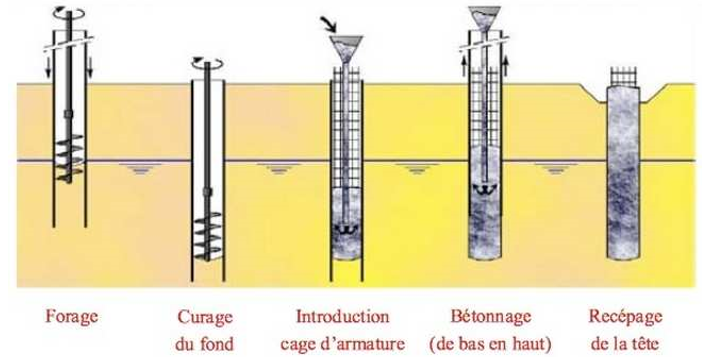
\includegraphics{Holeyman/images/H35.PNG}
            \caption{Pieu foré (exécuté par excavation du sol}
        \end{figure}
        
        \subsubsection{Pieux à refoulement limité ou à faible décompression du sol (groupe 2)}
        
        Ces pieux ont un degré de refoulement intermédiaire au groupe 1 et 2. 
        
        \begin{itemize}
            \item Soit ils sont installés par refoulement (groupe 1) mais le refoulement se produit au moyen d'une partie de la section apparente du pieu. Généralement des pieux métalliques tubulaire, des poutrelles H ou assemblé au départ de palplanches dont la section refoulée ne représente qu'une faible partie de la section circonscrite.
            \item Soit ils sont installés par extraction (groupe 3) mais comprennent des dispositions visant à corriger la compression du sol. Généralement des pieux forés à la tarière creuse continue à hélice réduite ou avec mise en suppression du béton.
        \end{itemize} 
        
        \subsubsection{Micro pieux (groupe 4)}
        
        Ce sont des pieux de diamètre inférieur à 250 mm. Ils comportent une armature centrale scellée dans un coulis de ciment. Servent en compression et en traction. Ils conviennent aux reprises en sous-oeuvre et aux travaux difficiles d'accès (Engin léger d'installation). 
        
    \subsection{Déterminer la capacité portante d'un pieu isolé sous la charge axiale}
    
        Dans un cas réel, on commence par effectuer un essai de mise en charge qui permet de mesurer l'enfoncement d'un pieu et d'en déterminer la courbe \textit{charge - tassement}. 
        
        \begin{figure}[h!]
            \centering
            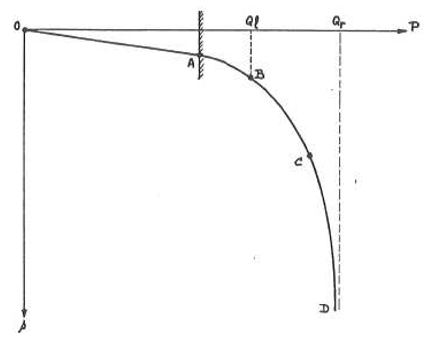
\includegraphics[scale=0.6]{Holeyman/images/H36.PNG}
            \caption{Allure de la courbe charge-tassement d’un pieu }
        \end{figure}
        
        \begin{itemize}
            \item OB: déformation pseudo élastique, au début (OA) le tassement est presque entièrement dû aux comportements élastiques du pieu et du sol.
            \item BC: déformation élastique du pieu et déplacement permanent irréversible se produit (correspond à un glissement du pieu par rapport au sol).
            \item CD: Zone de rupture, tassement augmente fortement voir indéfiniment pour un faible accroissement de charge appliquée.
        \end{itemize} 
        
        Dans certain cas, cette limite de rupture est très marquée, mais dans d'autre non. On définit alors une charge limite théorique conventionnelle en traçant une parallèle  à la droite caractérisant les faibles enfoncements à partir d'un point défini par un pourcentage du diamètre du pieu (Ex: 4, 10 ou 25\% du diamètre (pour le shéma $=$ 50mm)).
        
        \begin{figure}[h!]
            \centering
            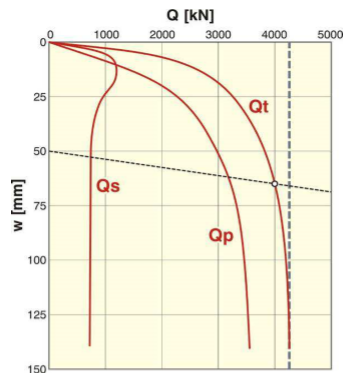
\includegraphics[scale=0.6]{Holeyman/images/H37.PNG}
            \caption{ Charge limite théorique conventionnelle }
        \end{figure}
        
        La figure ci-dessus donne un exemple de courbe de chargement d'un pieu de grand diamètre ($\phi = 1,25$m) moulé en place et de écomposition de la charge totale $Q_t$ en résistances mobilisées à la pointe $Q_p$ et au frottement latéral $Q_s$.
        
        On constate que le frottement latéral est entièrement mobilisé pour un enfoncement de $10-15$mm alors qu'il faut un tassement de l'ordre de $100-150$mm (soit dix fois plus grand) pour développer complètement la résistance à la base $Q_p$. Il résulte de ceci que si une structure peut tolérer un tassement de 10mm, il y correspond une charge de service de 2000 kN dont seulement 50\% provient de la pointe. Cette proportion évoluera en fonction de la charge totale appliquée en tête.
        
        On peu déduire la charge limite d'un pieu isolé d'un essai de mise en charge statique, d'un essai dynamique, des paramètres intrinsèques de cisaillement ou d'essais in situ. Les deux premières méthodes sont plus fiables mais plus coûteuses alors que les deux secondes, purement mathématiques, sont moins fiables (généralement réalisé en avant-projet).
        
        \subsubsection{dimensionnement par essai de mise en charge statique}
        
        Il s'agit d'un essai de charge-tassement. Graphiquement, en présence d'un pieu flottant la résistance due au frottement latéral devient plus ou moins constante lorsqu'on atteint des valeurs limites. En présence d'un pieu ou la résistance est principalement due à la base, cette résistance augmente continuellement avec l'enfoncement.
        
        Conventionnellement, on considère que la capacité portante d'un pieu est la charge provoquant un rapport de 10\% entre l'enfoncement de la tête du pieu ($S_0$) et le diamètre de la base ($D_b$). 
        
        \begin{center}
            $ \frac{S_0}{D_b} = 10\% $
        \end{center}
        
        \subsubsection{dimensionnement par essai dynamique}
        
        Cette procédure requiert un équipement spécifique de mesure. On laisse tomber d'une hauteur donnée sur la tête du pieu un mouton (insérer blague avec "méchoui"). On mesure la vitesse d'enfoncement du pieu et la contrainte qui lui est appliquée. On les interprète sur une courbe de chargement. 
        
        \begin{figure} [h!]
            \centering
            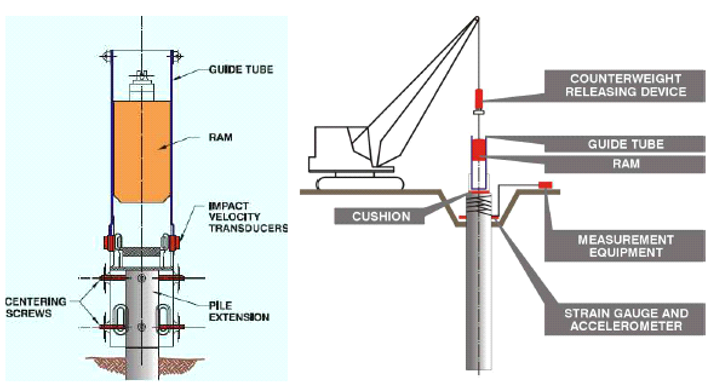
\includegraphics[scale=0.8]{Holeyman/images/H38.PNG}
        \end{figure}
        
        Il existe un procédé moins fiable qui consiste à enfoncer de manière permanente un pieu (appelé refus). On mesure sont enfoncement par rapport à l'impact et on en décuit la résistance du pieu.
        
        Le principe de base derrière cette méthode est que l'énergie résultant de la chute du mouton, diminué des pertes d'énergie correspondantes, est égale à l'énergie nécessaire pour faire pénétrer le pieu dans le sol. On exprime donc le travail du mouton diminué du travail perdu durant le choc, engrangé par les déformations élastique et du travail perdu pour d'autres causes est égal au travail net d'enfoncement du pieu. Cela forme une jolie formule qui a été interprétée par pleins d'auteurs qui ont bien-sûr pleins de réponses différentes sans que aucune d'entre elles ne soit convaincante (il s'agit pourtant bien d'une des méthodes les plus fiables!). En voici quatre des plus utilisées: 
        
        \begin{center}
        \begin{tabular}{c|c}
            $\eta_c \eta_i Mgh = \frac{1}{2} Q_d s_{el} + Q_d s$ \: \: \:
            &  $\eta_c$: efficacité de la chute [/]  \\
            &  $\eta_i$: efficacité de l'impact [/]  \\
            &  $M$: masse du mouton [Kg]  \\
            &  $h$: hauteur de la chute [m]  \\
            &  $S_{el}$: déplacement élastique [m]  \\
            &  $S$: déplacement permanent, refus [m]  \\
            &  $\mu = \frac{M}{M_p} \: M_p$: Masse du pieu [Kg]  \\
            &  $L$: longueur du pieu  \\
            &  $e$: coefficient de restitution du casque de battage  \\
            &  $C_1$ \& $C_2$: constante de Hiley  \\
            &  $Q_d$: résistance dynamique du pieu à l'enfoncement [kN]  
        \end{tabular}
        \end{center} 
        
        \begin{tabular}{c|c|c|c}
            Formule / coefficients \: \: & $\eta_c$ & $\eta_i$ & $s_{el}$ \\
            & & & \\
             Hollandaise  & 1 & 1 & 0 \\
             danoise  & $0,7 \to 1$ & $\frac{1}{1+\mu}$ & 0,6.$10^{-3}$ [L] \\
             Hiley  & $0,7 \to 1$ & $\frac{1+e_r^2\mu}{1+\mu}$ & $C_1 + \frac{Q_D L}{A_p E} + C_3$ \\
             Delmag & 1 & $\frac{1}{1+\mu}$ & $(\frac{2 \eta_c MghL}{A_pE})^\frac{1}{2}$
        \end{tabular}
        
        \subsubsection{Calcul selon la théorie classique de la mécanique des sols}
        
        On repart de l'équation de base: $Q_t = Q_p + Q_s$ 
        
        On peu l'écrire: 
        
        \begin{center}
        \begin{tabular}{c|c}
            $Q_t = q_{bu}A_b + q_{su}A_s$ \: \: 
            &  $q_{bu}$: résistance unitaire à la base (composante normale de la contrainte ultime)  \\
            &  $A_b$: la section de la base  \\
            &  $q_{su}$: le frottement latéral unitaire le long du fût (cisaillement)  \\
            &  $A_s$: surface latérale du fût  
        \end{tabular}
         \end{center} 
        
        On observe que la surface de la base est normale au vecteur déplacement du pieu (à la rupture) et que la surface latérale du fût lui est parallèle. 
        
        \underline{Frottement latéral unitaire $q_{su}$:} 
        
        \textbf{Pour les sols pulvérulent (c=0)} on calcule en condition drainé:
        
        \begin{center}
        \begin{tabular}{c|c}
            $q_{su} = \sigma'_h \tan \delta = K \sigma'_v \tan \delta $ \: \: \: & $\delta \le \phi $   
        \end{tabular}
        \end{center} 
        
        $K$ dépend du mode de mise en place du pieu et $\delta$ de la densité relative du sable et du matériau constituant le pieu. Cette approche s'utilise également pour des sols drainant lentement (limons, argile) pour autant que la sollicitation soit permanente.
        
        \textbf{Pour des sols cohérent} on considère que le frottement latéral est directement lié à la cohésion non drainée $c_u$ par la relation: 
        
        \begin{center}
            $q_{su} = \alpha C_u$
        \end{center} 
        
        On trouve $\alpha$ dans des abaques qui dépendent de la cohésion non drainée et du type de pieu. Cette approche s'applique à des sols non drainé, dont le drainage est très lent où pour des charges réputées transitoire .
        
        \underline{Résistance unitaire à la base $q_{bu}$:} (c'est encore un truc pas clair !!) 
        
        Il est possible de déterminer le pouvoir portant à sa base par analogie avec une semelle filante. On considère une paroi profonde de longueur infinie sur une profondeur $z$ dans un terrain caractérisé par $c'$, $\phi'$ et $\gamma'$. Par analogie avec la semelle filante, on suppose que la surface de glissement est composée de deux segments de droite d'une spirale logarithmique. Apparemment l'angle de la spiral devient dans ce cas-ci $\phi$ 
        
        On s'attend donc à trouver une équation du même type que pour une fonation superficielles:
        
        \begin{center}
        \begin{tabular}{c|c}
            $q_{bu} = c' N'_c + \sigma'_{vo} N'_q$ \: \: \: 
             &  $N'_q = K_p e^{2 \pi \tan \phi} = \tan^2 (\frac{\pi}{4} + \frac{\phi'}{2}) e^{2\pi \tan \phi'}$  \\
             &  $N'_c = \frac{N'_q-1}{\tan \phi'} $  \\
             &  $\sigma'_0$: contrainte de référence = contrainte effective à la profondeur de la base  \\
             &  $N'_{\gamma} = 0$ car la largeur est insignifiante par rapport à la profondeur  
        \end{tabular}
        \end{center}
        
        On trouve dans la littérature une grande variété d'expressions différentes pour $N'_q$ pour des pieux à refoulement. Elles constituent des valeurs très différentes en fonction du $\phi'$ utilisée. C'est pourquoi en règle générale on préfère se fier au résultats quantitatifs de la reconnaissance géotechnique (surtout en Belgique, France, Pays-Bas, ...). \textbf{On doit retenir que la taille du bulbe reste bien proportionnel à la taille du pieu}.
        
        \subsubsection{Calcul semi-empirique basé sur le CPT}
        
        Moyennant un changement d'échelle, on peut comparer un pieu au dispositif tige-cône d'un essai CPT. Il existe des méthodes pour en tirer des valeurs de résistance d'un pieu.
        
        \begin{center}
            $Q_{b,r} = q_{b,r} A_b$ \: \: \: (charge limite à la base)
        \end{center} 
        
        Il faut tenir compte de trois facteurs:
        \begin{itemize}
            \item la résistance en pénétration qui augmente en fonction de la profondeur (géré par une mise à l'échelle du problème) ($d_{g,d}$).
            \item introduction d'un coefficient propre au type de sol et type de pieu ($\alpha_d$).
            \item caractère fissuré du sol ($\epsilon_d$)
        \end{itemize} 
        
        On obtient une formule spécifique à la Belgique:
        
        \begin{center}
            $q_{b,r} = \alpha_b \epsilon_b d_{g,d} $
        \end{center} 
        
        \underline{Effet d'échelle:} 
        
        Sur base du diagramme de la résistance unitaire à la pointe $q_c$ relative à un sol composé de deux couches (faible résistance suivit de forte résistance). On constate que l'on ne peut mesurer la valeur de $q_c$ que lorsque le bulbe de refoulement a pu totalement se refouler dans la couche compacte. 
        
        \begin{figure}[h!]
            \centering
            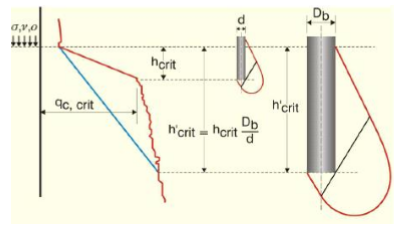
\includegraphics{Holeyman/images/H39.PNG}
            \caption{Résultat d’un essai CPT et sa mise à l’échelle du pieu}
        \end{figure}
        
        \begin{center}
        \begin{tabular}{cc}
            $d_{g,d} = q_c$ \: \: \: 
                &  (uniquement dans la seconde couche)  \\
            $h'_{crit} = h_{crit} \frac{d_b}{d}$ 
                &  hauteur à laquelle la relation précédente est mesurée  \\
                 &  ($d_b$: diamètre du pieu et $d$ celui de la tige de l'essai)   
        \end{tabular}
        \end{center} 
        
        La difficultée réside dans le fait que le diagramme est généralement irrégulier, la valeur de $d_{g,d}$ n'est donc pas directement lisible sur le diagramme. Il existe plusieurs méthodes pour calculer $d_{g,d}$.
        
        \underline{Méthode hollandaise:} 
        
        Begeman considère une surface de rupture définie par une spirale logarithmique correspondant à une valeur représentative de l'angle $\phi$ des sables hollandais. Il tient compte des valeurs de $q_c$ comprise entre $h_s$ et $h_i$. Le pouvoir portant $d_{g,d}$ est défini comme une moyenne arithmétique:
        
        \begin{center}
            $d_{g,d} = \frac{d_{g,d,s} + d_{g,d,i}}{2}$
        \end{center} 
        
        $d_{g,d,s}$ et $d_{g,d,i}$ sont calculé par la moyenne des valeurs de $q_c$ sur leur différence de hauteur respective avec la base (voir shéma ci-dessous). Donnons quelques exemples: 
        
            \begin{multicols}{3}
            
                \begin{figure}[h!]
                \center
                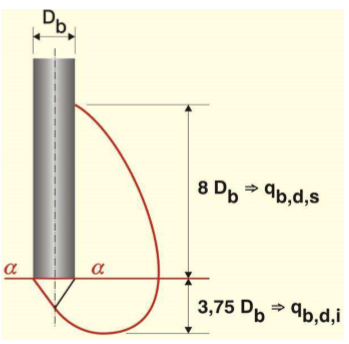
\includegraphics[scale=0.6]{Holeyman/images/H40.PNG}
                \caption{Zones d’influence supérieure et inférieure selon la méthode hollandaise}
                \end{figure}
            
            \vfill\null\columnbreak
            
                \begin{figure}[h!]
                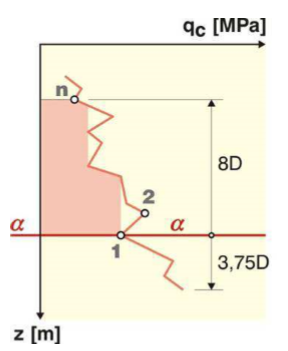
\includegraphics[scale=0.6]{Holeyman/images/H41.PNG}
                \caption{Rabotage de qc en zone supérieure }
                \end{figure}
                
            \vfill\null\columnbreak
            
                \begin{figure}[h!]
                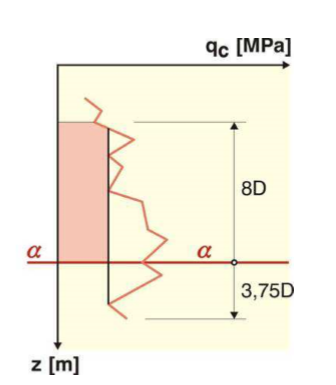
\includegraphics[scale=0.6]{Holeyman/images/H42.PNG}
                \caption{Rabotage de qc depuis zone inférieure}
                \end{figure}
                
            \end{multicols}
        
        Supposons que toutes les valeurs de $q_c$ soient supérieur à la valeur correspondant au niveau de la base. Les $q_c$ sous ce niveau sont supérieur aux valeurs de $q_c$ au point 1. On prend donc en compte la valeur de $q_c$ au point 1. La valeur de $q_c$ au point 2 étant supérieur à celle du point 1, on supprime le triangle et on utilise la valeur de $q_c$ au point 1 pour le point 2 (c'est une méthode qui s'apparente à du rabotage). On continue ainsi en remontant la courbe. On fait pareil dans l'autre sens. Une fois les $n$ valeurs de $q$ (éventuellement modifiée) connues, on peu calculer:
        
        \begin{center}
            $ d_{g,d,s} = \frac{\frac{q_{c,i}}{2}+\sum_{j=2}^{n-1}q_{c,j}+\frac{q_{c,n}}{2}}{n-1}$
        \end{center} 
        
        La méthode hollandaise donne généralement d'assez bon résultats sauf lorsque la base du pieu se trouve figé dans une couche de sol relativement compacte. Dans ces circonstances elle conduits à des valeurs dangereusement optimistes.
        
        \underline{Méthode belge:} 
        
        Elle se base sur les lois de similitude et tient compte de l'effet d'échelle ainsi que de l'influence de la présence d'une couche de moindre résistance sous une couche compacte. La complexité du calcul implique généralement le recours à un ordinateur. Elle est très précise. 
        
        \underline{Sécurité:} 
        
        La charge utile d'un pieu ne peut s'approcher de sa charge limite. Il faut respecter des critères. Dans l'approche moderne, les incertitudes ne sont pas gérées via un seul coefficient de sécurité global mais plutôt introduites via des coefficients de sécurité partiels.
        
    \subsection{Autres considérations}
    
        \subsubsection{Frottement négatif}
        
        Lorsqu'on a affaire à un pieu travaillant principalement à la pointe et que le sol entourant le pieu est amené à assumer une charge, le terrain avoisinant le pieu peu tasser plus que le pieu et créer un frottement latéral dirigé vers le bas. C'est le frottement négatif. On le redoute lorsqu'un remblai est mis en place sur des couches compressibles traversé par des pieux.
        
        Le frottement négatif est très dangereux si on n'en tient pas compte, puisqu'au lieu de soutenir le pieu, il a tendance à le charger. En outre il augmente l'effort axial maximum supportable par le pieu.
        
        Le frottement négatif maximal $G_f$ peut être évalué par la relation suivante:
        
        \begin{center}
        \begin{tabular}{c|c}
             $G_f = P \int_{-H}^h K \tan \delta \sigma'_v \, \mathrm{d}z $ \: \: \:
             &  p: périmètre du pieu   \\
             &  H: hauteur du remblai  \\
             &  h: hauteur d'action du remblai (couche compressible)  \\
             &  $\sigma'_v$: contrainte verticale (+effet d'accrochage)  
        \end{tabular}
        \end{center} 
        
        Les valeurs du terme $K \tan \delta$ sont disponible dans des tables.
        
        Le frottement négatif n'affecte que la partie supérieur du fût, la partie inférieur restant soumise au frottement positif. 
        
        \underline{Tassement un peu isolé:} 
        
        Prédire le tassement d'un pieu est difficile pour diverse raison:
        \begin{itemize}
            \item Il faut connaître la répartition réelle de charge appliquée entre la base et la tête.
            \item Il faut connaître la constante de compressibilité du terrain.
            \item La mise en place influence les caractéristique du sol en présence.
        \end{itemize} 
        
        Plusieurs méthodes d'estimation sont basées sur l'établissement des équations d'équilibre du pieu découpé en $n$ éléments. On fait les hypothèses suivante: 
        \begin{itemize}
            \item Symétrie des sollicitation (contraintes de déformations par rapport à l'axe du pieu supposé cylindrique).
            \item Contrainte axiale uniformément répartie sur une section horizontale du pieu.
            \item Le poids du pieu correspond au poids de la colonne de terre enlevée.
        \end{itemize} 
        
        \begin{figure}[ht]
            \centering
            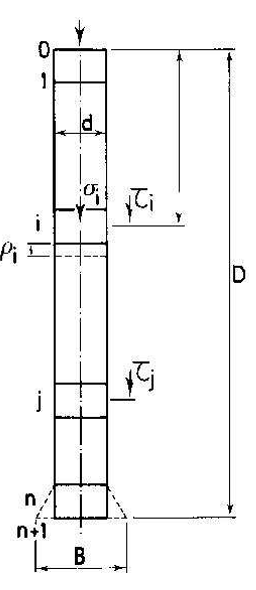
\includegraphics[scale=0.8]{Holeyman/images/H43.PNG}
            \caption{« Découpage » d’un pieu en tronçons }
        \end{figure}
        
        On définit:
        
        \begin{itemize}
             \item D: longueur du pieu
             \item $\tau$: contrainte tangentielle de frottement latéral 
             \item B: diamètre de la base éventuellement élargie 
             \item e: élancement du pieu ($\frac{D}{d}$) 
             \item $E_p$: module de déformation du pieu 
             \item $E_s$: module de déformation du sol 
             \item K: raideur relative du pieu-sol  
             \item $\nu_s$: coefficient de poisson du sol  
             \item Q: charge appliquée en tête de pieu  
             \item d: diamètre du pieu  
             \item i: point ou il y a un déplacement vertical  
             \item v: le déplacement vertical  
             \item $\sigma$: contrainte axial dans le pieu  
             \item j: point ou il y a une contrainte  
        \end{itemize}
        
        \underline{Méthode de T-z:} 
        
        L'équilibre vertical s'établi comme suit: 
        
        \begin{center}
        \begin{tabular}{c|c}
            $(\sigma_{z,j} - \sigma_{z,j-1}) S = \tau_{z,j} X h_i$ \: \: \:
             &  S: section  \\
             &  x: périmètre  \\
             &  h: hauteur  \\
             &  $\sigma$: la contrainte axial  
        \end{tabular}
        \end{center}   
        
        On utilise ensuite la loi de Hooke pour calculer le raccourcissement $dw_z$ du tronçon $i$:
        
        \begin{center}
            $dw_z = \frac{dz}{E_p} \frac{\sigma_{z,j-1} + \sigma_{z,j}}{2} = \frac{dz}{E_p} \frac{\sigma_{z,j-1}(\sigma_{z,j}-\sigma_{z,j-1}}{2}$
        \end{center}
        
        On résout le système et on obtient:
        
        \begin{center}
            $dw_z = \frac{dz}{E_p} [\sigma_{z,j-1} + \tau_{z,j} \frac{\chi^{dz}}{2\Omega}]$
        \end{center} 
        
        \underline{Méthode du milieu continu:} 
        
        On introduit ici un nouveau coefficient, $\mu_{ij}$, le coefficient de Midlin. Il permet d'évaluer le déplacement vertical dans un espace semi-élastque et homogène:
        
        \begin{center}
            $p_{ij} = \mu_{ij} Q_j$
        \end{center} 
        
        En intégrant cette expression sur une géométrie cylindrique tout en respectant les conditions de compatibilités. Ce calcul a été effectué pour un pieu flottant et un pieu portant à sa base. L'équation donnant le tassement en tête de pieu ainsi obtenue revêt une forme simple mais dont le coefficient fait appel à une série d'abaques:
        
        \begin{center}
        \begin{tabular}{c|c}
             $p = Q \frac{I}{E_s} b $  \: \: \:
             &  Pieux flottants: $I = I_0 R_k R_v R_h $  \\
             &  Pieux portants: $I = I_0 R_k R_v R_b $  
        \end{tabular}
        \end{center}
        
        \begin{itemize}
            \item $I_0$ est le coefficient d'influence d'un pieu infiniment rigide dans un semi-espace avec $\nu=0.5$. On le trouve dans un abaque en fonction de l'élancement pour différentes valeurs d'élargissement relatif de la base.
            \item $R_k$ est un coefficient majorant prenant en compte la compressibilité relative du pieu-sol ($\frac{E_p}{E_s}$).
            \item $R_v$ est un coefficient minorant prenant en compte le coefficient de poisson du sol.
            \item $R_h$ est un coefficient minorant dans le cas où le massif semi)infini se limite à une couche d'épaisseur donnée reposant sur un substratum incompressible.
            \item $R_b$ est un coefficient minorant tenant compte de la valeur relative de la couche portante
            \item $R_b$ ... Ce coefficient est représenté aux figures ci-dessous respectivement pour différents élancement $e = \frac{D}{b}$.
        \end{itemize}
        
        \subsubsection{Groupe de pieux}
        
        Pour estimer de manière approchée le tassement d'un groupe de pieux qui ne sont pas portant à la base, Terzaghi suppose que le tassement du groupe est égal à celui d'un radier équivalent situé à une profondeur égale à $\frac{2}{3}$ de la "fiche" (profondeur) et dont la surface est déterminée par la pente de répartition $\frac{1}{2}$. Le tassement du groupe est alors donné par:
        
        \begin{center}
        \begin{tabular}{c|c}
             $W_g = W_f + \Delta w $ \: \: \:
             &  $W_f$: tassement du radier équivalent  \\
             &  $\Delta w$: raccourcissement des pieux (au-dessus du radier)  
        \end{tabular}
        \end{center} 
        
        \begin{figure}[h!]
            \centering
            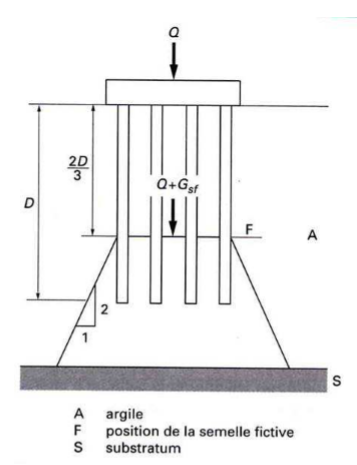
\includegraphics[scale=0.8]{Holeyman/images/H44.PNG}
            \caption{Méthode du radier équivalent }
        \end{figure}

        Dans le cas ou le pieu traverse une fine couche superficielle de faible résistance, on ne la considère pas. Dans le cas d'une fondation profonde à base portante, on considère exclusivement la base des pieux, le radier équivalent occupe alors la surface d'appui du groupe, sans pente de répartition.
        
\section{Ouvrage de soutènement}

    Dénition: un ouvrage de soutènement est un dispositif structurel dont la fonction est de soutenir le sol sur une hauteur donnée afin de réaliser une différence de niveau sur une distance réduite voire nulle.
    
    \subsection{Quelques normes}
    
        Il en existe trois formes principales: mur poids, mur équerre ou écran. Ils sont prévu pour pouvoir résister aux efforts provenant du massif de sol soutenu. Nous allons dans un premier temps évaluer les efforts auxquels ils sont soumis. Ensuite nous vérifierons leurs états d'équilibre compte tenu des réactions disponibles. 
        
        \begin{figure}[h!]
            \centering
            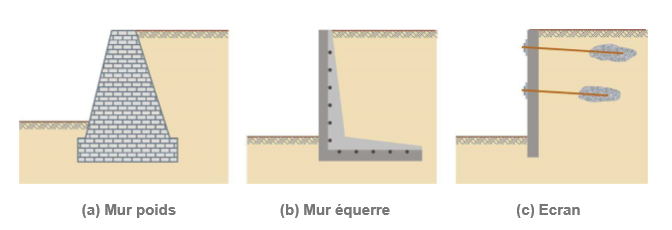
\includegraphics[scale=0.8]{Holeyman/images/H45.PNG}
            \caption{Principaux types d’ouvrages de soutènement }
        \end{figure}
        
        Soit une surface en contact entre un ouvrage de soutènement et le sol. La contrainte exercée par le sol sur l'ouvrage peut être décomposée en une contrainte normale effective $\sigma'$ (positive en compression) et une contrainte tangentielle $\tau$ (positive lorsque le massif tourne dans le sens anti-horlogique). 
        
        On défini trois angles:
        \begin{itemize}
            \item $i$ entre l'horizontal et la face du terrain-plein soutenu.
            \item $\beta$ entre la vertical et la surface de contact de l'ouvrage de soutènement avec les terres soutenues.
            \item $\sigma$ entre la normale à cette surface et la contrainte totale.
        \end{itemize} 
        
        \begin{figure}[h!]
            \centering
            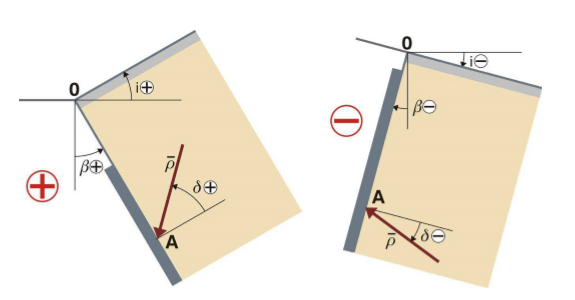
\includegraphics[scale=1]{Holeyman/images/H46.PNG}
            \caption{Conventions }
        \end{figure}
        
    \subsection{Pression des terres sur un ouvrage de soutènement}
    
        On ne s'intéresse ici qu'à des cas ou la direction de la surface de contact ouvrage-sol ne s'éloigne pas trop de la verticale. 
        
        Le problème est le suivant: si une paroi subverticale de forme quelconque fait partie d'un ouvrage subissant des déplacements, en contact avec un massif au sol constitué de couches différentes et limitée par un terre-plein de forme quelconque sur laquelle est appliquée une charge quelconque, quelle est la grandeur et la répartition des contraintes sur cette paroi? 
        
        Plusieurs théorie peuvent être avancées pour résoudre ce problème.
        
        \subsubsection{Méthode de Coulomb}
        
        Coulomb recherche un extremum, il établi une surface de glissement et suppose que le massif de sol situé au-dessus de celle-ci, est un corps rigide. L'effort agissant sur le mur et dont la réaction met le massif à l'équilibre dépend de la surface de glissement spéculée. La plus défavorable étant celle qui donne une valeur maximale de poussée ou minimale de butée. 
        
        Nous allons analyser le cas suivant: soit un ouvrage de soutènement AB faisant un angle $\beta$ avec la verticale et un terrain-plein faisant un angle $i$ avec l'horizontale (on considère un sol pulvérulent qui n'est défini que par $\gamma$ et $\phi$). On donne une surface AC orienté d'un angle $\theta$. 
        
        \begin{figure}[h!]
            \centering
            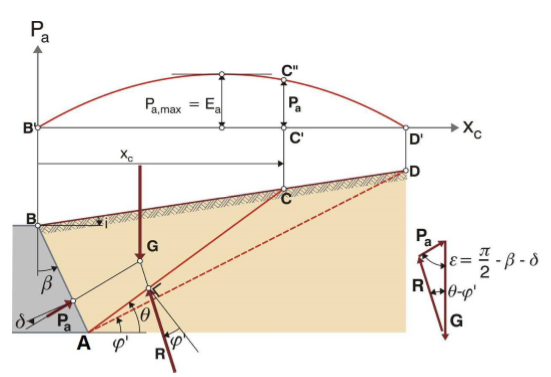
\includegraphics[scale=1]{Holeyman/images/H47.PNG}
            \caption{Méthode de Coulomb (résolution) }
        \end{figure}
        
        Il y a trois forces en présence:
        \begin{itemize}
            \item $P_a$: la réaction du mur (formant un angle $\sigma$ avec la normale de la paroi).
            \item $G$: Le poids du massif supérieur à la surface de glissement AC.
            \item $R$: la réaction le long de la surface de glissement faisant un angle $\phi'$ avec la normale
        \end{itemize} 
        
        On trouve un maximum $P_{a,max} = E_a$ pour une droite de glissement AC entre les positions AD et AB.
        \begin{itemize}
            \item si $C=D$ alors on est à la limite d'équilibre sur AD $\to \: P_a=0$
            \item si $C=B$ alors $G=0 \: \to \: P_a = 0$
        \end{itemize} 
        
        La recherche de $P_{a,max}$ peut se faire soit graphiquement:
        
        Si on porte $P_a$ en fonction de l'abscisse du point C, on obtient une courbe B'C''D'. On définit la tangente horizontale à cette courbe et on obtient le point maximum soit $E_a$. On trace ensuite la surface de glissement correspondante. 
        
        Le problème peut être résolu analytiquement (c'est un brin géométrique, pour la voir p5 du pdf "Mur de soutènement"). 
        
        Il faut définir l'angle entre chacun des vecteurs forces et les simplifier au maximum. On obtient les valeurs écrites ci-dessous dans le polygone des forces. Pour l'angle $\alpha$, soit celui entre $P_a$ et $R$: $\alpha = \frac{\pi}{2} + \beta + \sigma - \theta + \phi'$ 
        
        Ensuite on trace sur la figure les droites $\bar{BF} = a$ et $\bar{CE} = x$ ainsi que la droite $\delta$ passant par A faisant toutes trois un angle $\epsilon$ avec AD ($\epsilon = \frac{\pi}{2} - \beta - \delta$). Les longueur formée $\bar{AF}$, $\bar{AE}$ et $\bar{ED}$ valent respectivement d, y et b (ne pas oublier de simplifier la valeur de tous les angles formés). 
        
        \begin{figure}[h!]
            \centering
            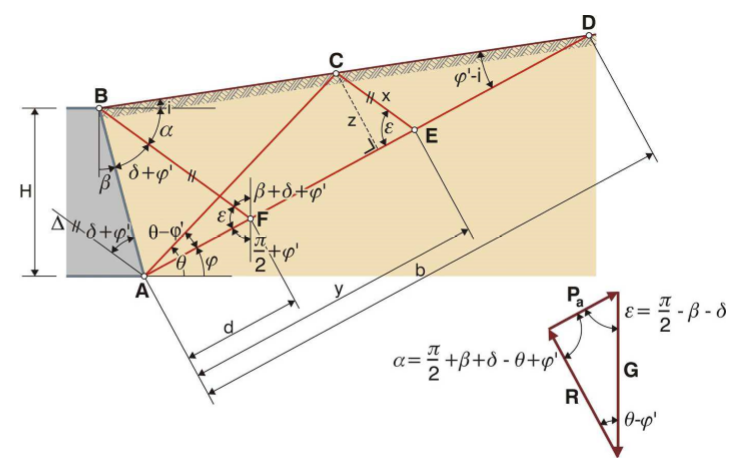
\includegraphics[scale=1]{Holeyman/images/H48.PNG}
            \caption{ Méthode de Coulomb (résolution analytique) }
        \end{figure}
        
        Observation:
        \begin{itemize}
            \item Les longueurs a, b et d sont constantes tandis que x et y varie selon $\theta$.
            \item le triangle ACE est semblable au polygone des forces: $P_a y = G x$.
            \item Le poids de G est proportionnel au triangle ABC: $S_{ABC} \gamma = G$.
            \item $S_{ABC} = S_{ABD} - S_{ACD}$
            \item BDF et CDE sont semblable $\to$ il y a une expression de x en fonction de y.
        \end{itemize} 
        
        Grâce à ces observation on trouve une équation de $P_a$ qui ne dépend plus que de x. On cherche l'optimum. Une fois simplifié on obtient une expression de $x_{max}$.
        
        Ce $x_{max}$ permet de trouver soit $y_{max}$, soit $P_{a,max}$. Une fois simplifié, nous avons x, y et $P_a$ estimé en fonctions constantes.
        
        \begin{center}
        \begin{tabular}{ccc}
             $x_M = a \frac{1}{1+\sqrt{\frac{d}{b}}}$ \: \:
             & $y_M = \sqrt{bd}$ \: \: \:
             & $E_a = P_{a,max} = \frac{1}{2} \gamma \sin \epsilon a^2 \frac{1}{[1+\sqrt{\frac{d}{b}}]^2}$ 
        \end{tabular}
        \end{center} 
        
        Il reste a exprimer ces constantes en fonction des données du problème. On fait un peu de trigonométrie et de géométrie sur les triangles ABF et ABD. On introduit toutes les jolies équations trouvées dans la solution et on obtient:
        
        \begin{center}
            $E_a = \frac{1}{2} \gamma H^2 K_a $
        \end{center} 
        
        $K_a$ dépend des valeurs de $\beta$ et $i$ du problème initial, il existe des tables pour ne plus devoir le calculer. Coulomb à donné une formule pour l'estimer plus facilement selon certaines hypothèses: 
        \begin{itemize}
            \item La surface de glissement potentielle est un plan.
            \item La paroi de l'ouvrage de soutènement est verticale ($\beta = 0$).
            \item Le terre-plein est horizontal ($i = 0$).
            \item L'ouvrage de soutènement est parfaitement lisse ($\sigma = 0$). Cela signifie que la poussée est horizontale.
        \end{itemize} 
        
        Il a obtenu la formule suivante : $K_a = \tan^2(\frac{\pi}{4}-\frac{\phi'}{2})$ 
        
        Hors hypothèse: $K_a = \frac{\cos^2(\phi'-\beta)}{\cos^2\beta \cos(\beta+\delta)[1+\sqrt{\frac{\sin(\phi'-i) \sin(\phi'+\delta)}{\cos(\beta-i)\cos(\beta+\delta}}]^2}$
        
        \subsubsection{Méthode de Cullmann}
        
        C'est une méthode graphique:
        \begin{itemize}
            \item Tracer la droite d'orientation $\delta$ et la droite AD d'inclinaison $\phi'$.
            \item Considérer une surface de glissement AC.
            \item Porter le long de AD un segment AP proportionnel au poids du massif ABC.
            \item Tracer en P une droite parallèle à $\delta$ qui croise AC en M.
            \item Observer que le polygone des forces et le triangle APM sont semblable $\to$ PM proportionnel à $P_a$.
        \end{itemize} 
        
        Il procède ainsi pour plusieurs lignes de glissement AC, la courbe formée par l'ensemble des point M est appelée courbe de Cullmann. Il faut tracer une tangente à cette courbe parallèle à AD. On trouve M et donc P. Finalement, on trace AMC et on obtient la ligne de glissement provoquant $E_a$. 
        
        \begin{figure}[h!]
            \centering
            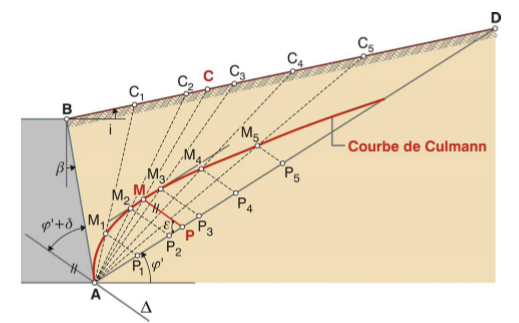
\includegraphics[scale=1]{Holeyman/images/H49.PNG}
            \caption{Courbe de Culmann}
        \end{figure}
        
        \underline{Surcharge répartie:} 
        
        Il se peut que le massif soit chargé d'une charge uniformément répartie p. La valeur de G va évoluer: 
        \begin{center}
        \begin{tabular}{c|c}
            $G_1 = G + P \bar{BD}$ \: \: \: &  $\bar{BD}$ longueur de surface uniformément chargée 
        \end{tabular}
        \end{center} 
        
        En changeant la valeur de G dans la méthode de Coulomb (étape 2) et en l'insérant dans l'équation de $E_a$ trouvé précédemment, on obtient une nouvelle équation:
        
        \begin{center}
            $E_{a,p} = \frac{1}{2} \gamma H^2 K_a + \frac{P}{h} H^2 K_a$
        \end{center} 
        
        On peut y changer la valeur de H en fonction des données du problème par trigonométrie. 
        
        \underline{Surcharge ponctuelle:} 
        
        Dans le cas d'une charge ponctuelle on aura recours à la méthode graphique de Cullmann. En envisageant AC' et AC'' qui encadre la charge ponctuelle, on aura une discontinuité dans la courbe. La tangante reste aisément traçable et donc la valeur de $E_a$ facilement déductible.
        
        \subsubsection{Théorème de Rankine}
        
        La méthode de Rankine est basée sur un mécanisme de rupture totalement différent de celui de Coulomb. Elle considère chaque point du massif à la limite de l'équilibre, la plasticité est donc distribué dans le massif (Rupture zonale). cette méthode est étudié dans un autre chapitre (équilibre limite des massifs de sol). Notons simplement que cette méthode se réfère aux cercles de Mohr. La contrainte agissant sur le plan incliné de $\beta$ par rapport à la verticale est fixé par les contraintes du cercle tangent aux droites de rupture. L'utilisateur n'est plus libre d'une valeur de $\sigma$ telle que permise par Coulomb.
        
        \subsubsection{Méthode de Caquot et Kérisel}
        
        La méthode de Caquot et Kérisel est une amélioration du théorème de Rankine qui permet de garder la liberté de $\sigma$ tout en incorporant une rupture zonale. On trouve leurs résultats sous forme de tables donnant les valeurs de $K_a$ et $K_p$ en fonction de $i$, $\beta$ et $\sigma$. 
        
        Ces tables sont généralement utilisée pour les murs poids (écrans, palplanches,...) lorsque $\beta$ et $\sigma$ valent 0.
        
    \subsection{Murs poids et murs équerre}
    
        La stabilité d'un mur poids est assuré par son poids propre, alors que celle du mur équerre par le poids des terres reposant sur la semelle.
        
        \subsubsection{Conditions de stabilité des murs de soutènement}
        
        Il faut respecter différent aspect:
        \begin{itemize}
            \item Glissement: le mur ne peut pas être sujet à des translation horizontale.
            \item Renversement: pas de basculement autour d'un point de sa base.
            \item Portance: sol capable de supporter le poids, pas de tassement trop important.
            \item Organique: pas de rupture intrinsèque.
            \item Grand glissement: vérifier qu'une ligne de rupture ne puisse se fourmer sous le mur de soutènement.
        \end{itemize} 
        
        \subsubsection{Sollicitations sur un mur poids}
        
        \begin{multicols}{2}
        
        \begin{figure}[h!]
            \centering
            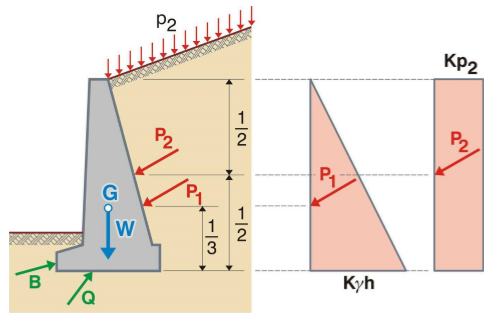
\includegraphics{{Holeyman/images/H50.PNG}}
            \caption{Sollicitations sur un mur poids }
        \end{figure}
                
        \begin{tabular}{c|c} 
            \: \: \: \: \: \: \: \:&  w: le poids propre du mur  \\
            &  B: réaction de butée du sol \\
            &  Q réaction du sol sous la semelle \\
            &  $P_1$: poussé des terres (poids propre) \\
            &  $P_2$: poussé des terres (surcharge $P_2$) 
        \end{tabular}
        
        \end{multicols}
        
        La force B se situe du côté sécurité car elle s'oppose au déplacement naturel, elle est généralement pas prise en compte dans les calculs de sécurité (la négligé rend le calcul défavorable, on obtient une marge de sécurité). De plus, le mur poids n'étant pas enfoncé profondément, il y a un risque d'excavation de terres et donc disparition de cette force B.
        
        Si on suppose un sol pulvérulent ($c'=0$) et non saturé ($u=0$), la poussée des terres pour une hauteur donnée s'appliquera perpendiculairement au mur.
        
        \begin{center}
        \begin{tabular}{cc}
             $P_1 = \int_0^h\bar{\rho_1}(z) dz = \int_0^h K_a \gamma zdz = K_a \gamma \frac{h^2}{2}$ \:
             &  $P_2 = \int_0^h\bar{\rho_2}(z) dz = \int_0^h K_a \gamma p_2 dz = K_a p_2 h $ 
        \end{tabular}
        \end{center} 
        
        $P_1$ s'applique au centre de gravité du triangle de terre, soit $h = \frac{H}{3}$, $P_2$ s'exprime à mi-hauteur $h=\frac{H}{2}$. Leur orientation dépend de l'angle $\sigma \le \phi$ adopté. 
        
        \subsubsection{Stabilité des murs de soutènement}
        
        La stabilité d'un ouvrage s'est développée au fil du temps en observant les échecs du passé. Grâce au progrès apporté dans la théorie de la plasticité, on peu observer que quelque soit la rupture rencontrée, il s'agit d'un problème de dimensionement des fondations du mur. 
        
        \underline{Stabilité au renversement:} 
        
        Il s'agit du rapport du moment des actions stabilisatrices sur le moment des actions promouvant le renversement. 
        
        Le choix du pivot déterminera le caractère stabilisant ou déstabilisant des actions. La méthode classique consiste à utiliser le point le plus en aval et de fixer un coefficient de sécurité de 1,5. 
        
        \underline{Stabilité au glissement sur la base:} 
        
        On considère la résultante des actions W, P et U vis à vis de la direction de glissement éventuel (donc selon ses composantes N et T au plan de glissement envisagé). 
        \begin{center}
        \begin{tabular}{cc|c}
             $N = W + (P_1 + P_2) \sin (\sigma + \beta)$ \:
             &  $T = (P_1 + P_2) \cos (\sigma + \beta)$ \:
             &  $\phi$ angle de frottement interne au sol  \\
             & &  $\sigma$ frottement fondation-sol, vaut habituellement $\frac{2\phi}{3}$  
        \end{tabular}
        \end{center} 
        
        \begin{center}
            $FS_g = \frac{N}{T} \tan \sigma   \ge 1.5$
        \end{center} 
        
        \underline{Stabilité à la portance:} 
        
        \underline{Stabilité organique:} 
        
        Consiste à vérifier si le matériau est capable de résister aux contraintes développées. On utilise pour ça la notion de ligne de poussée ou la théorie des poutres (dans le cas du béton armé). 
        
        \underline{Grand glissement:} 
        
        Il s'agit ici d'un mécanisme général de rupture de talus englobant le mur et une zone de sol attenante. Il faut étudier la stabilité du talus et non du mur pour cette vérification. 
        
        \begin{figure}[h!]
        \underline{Pré-dimensionnement:} 
        
        Les vérifications détailles ci-dessus ne peuvent se faire que sur base d'un mur dont la géométrie est définie. Elles permettent par raffinement successifs d'arriver à une conception sécuritaire et économique. La géométrie de départ est inspiré de conception type: 
        
            \centering
            \includegraphics{Holeyman/images/H51.PNG}
            \caption{ Proportions utiles au pré-dimensionnement d’un mur-poids (maçonnerie, empierrements, béton non armé) }
        \end{figure}
        
        
